\documentclass[master=cws,masteroption=gs]{kulemt}
\setup{title={Schaalbare genoomanalyse met NoSQL- databases},
		author={Brecht Gossel\'e},
		promotor={Prof. Dr. Roel Wuyts},
		assessor={},
		assistant={Prof. Dr. Roel Wuyts}}
\setup{filingcard,
		translatedtitle=Scalable genome analysis with NoSQL databases,
		udc=,
		shortabstract={Here comes a very short abstract, containing no more than 500 words. \LaTeX\ commands can be used here.}}
		
\usepackage{url}
\usepackage{graphicx}
\usepackage{booktabs}
\graphicspath{ {afbeeldingen/} }
\usepackage[dvipsnames]{xcolor}
\usepackage{changepage}
\usepackage{listings}
\usepackage[final]{pdfpages}
\usepackage{lscape}
\lstset{basicstyle=\footnotesize, showspaces=false, showstringspaces=false, keywordstyle=\color{blue}, stringstyle=\color[RGB]{26,196,8}}
\usepackage[pdfusetitle,colorlinks,plainpages=false]{hyperref}

\begin{document}

\begin{preface}
\end{preface}

\tableofcontents

\begin{abstract}
\end{abstract}


\mainmatter

\chapter{Inleiding}
\label{inleiding}

\section{Probleemstelling}

Wetenschappelijke vooruitgang heeft ervoor gezorgd dat de kost om genomen te sequencen het afgelopen decennium exponentieel gedaald is, sinds 2008 zelfs aan een hogere snelheid dan de evolutie volgens de wet van Moore \cite{wetterstrand_sequencing_cost}. Dit is duidelijk zichtbaar op de grafiek in figuur \ref{sequencing_cost}. In allerhande soorten biologisch, medisch en pharmaceutisch onderzoek worden dan ook genomen van meer en meer organismen gesequenced en dit genereert enorme hoeveelheden data. Ter illustratie: de \textit{whole genome sequencing pipeline} van het Broad Institute \cite{broad_institute}, een referentie in het veld, genereert bij het sequencen van 1 volledig menselijk genoom in de orde van 3TB aan tussentijdse data. Het eindresultaat is 50 GB gecomprimeerde data voor 1 menselijk genoom bij 50x \textit{coverage} (een maat voor de resolutie \cite{coverage_definition}). Naarmate genomen van miljoenen mensen en andere levende wezens geanalyseerd en opgeslagen worden, vereist deze evolutie steeds betere schaalbaarheid, responstijd, en parallellisering voor de opslag en verwerking van deze data.\\

Een logische stap is om deze problemen aan te pakken met grote verdeelde computersystemen, zogenaamde \textit{high performance computing systems} of \textit{supercomputers}. Het Exascience Life Lab van imec, Intel, Janssen Pharmaceutica en de 5 Vlaamse universiteiten verricht specifiek onderzoek naar de toepassing van supercomputers om het genoomsequencingproces te versnellen \cite{lifelab_bwa}\cite{exascience_life_lab}.\\
De snel toegenomen populariteit van webdiensten als sociale netwerken zadelde webservice-leveranciers op met een gelijkaardige explosie aan data. Om deze zogenaamde Big Data \cite{mashey1997big} adequaat te beheren, volstaan traditionele relationele DBMS niet meer. Daarom hebben grote webbedrijven zoals Google, Amazon en Facebook nieuwe opslagtechnieken ontwikkeld die voldoen aan de vereisten qua incrementele schaalbaarheid, lage responstijden en hoge beschikbaarheid \cite{baker2011megastore}. Dit heeft vele zogenaamde NoSQL ('Not only SQL') databases voortgebracht, die het rigide relationele datamodel inruilen voor betere schaalbaarheid en gemakkelijkere distributie van de data. Daarnaast is er ook de recentere opkomst van NewSQL-systemen: deze trachten de schaalbaarheid, distributie en fouttolerantie van NoSQL-systemen te combineren met het relationele datamodel en de bijhorende SQL-query interface en sterke garanties op gebied van concurrency en consistentie.

\begin{figure}[h!]
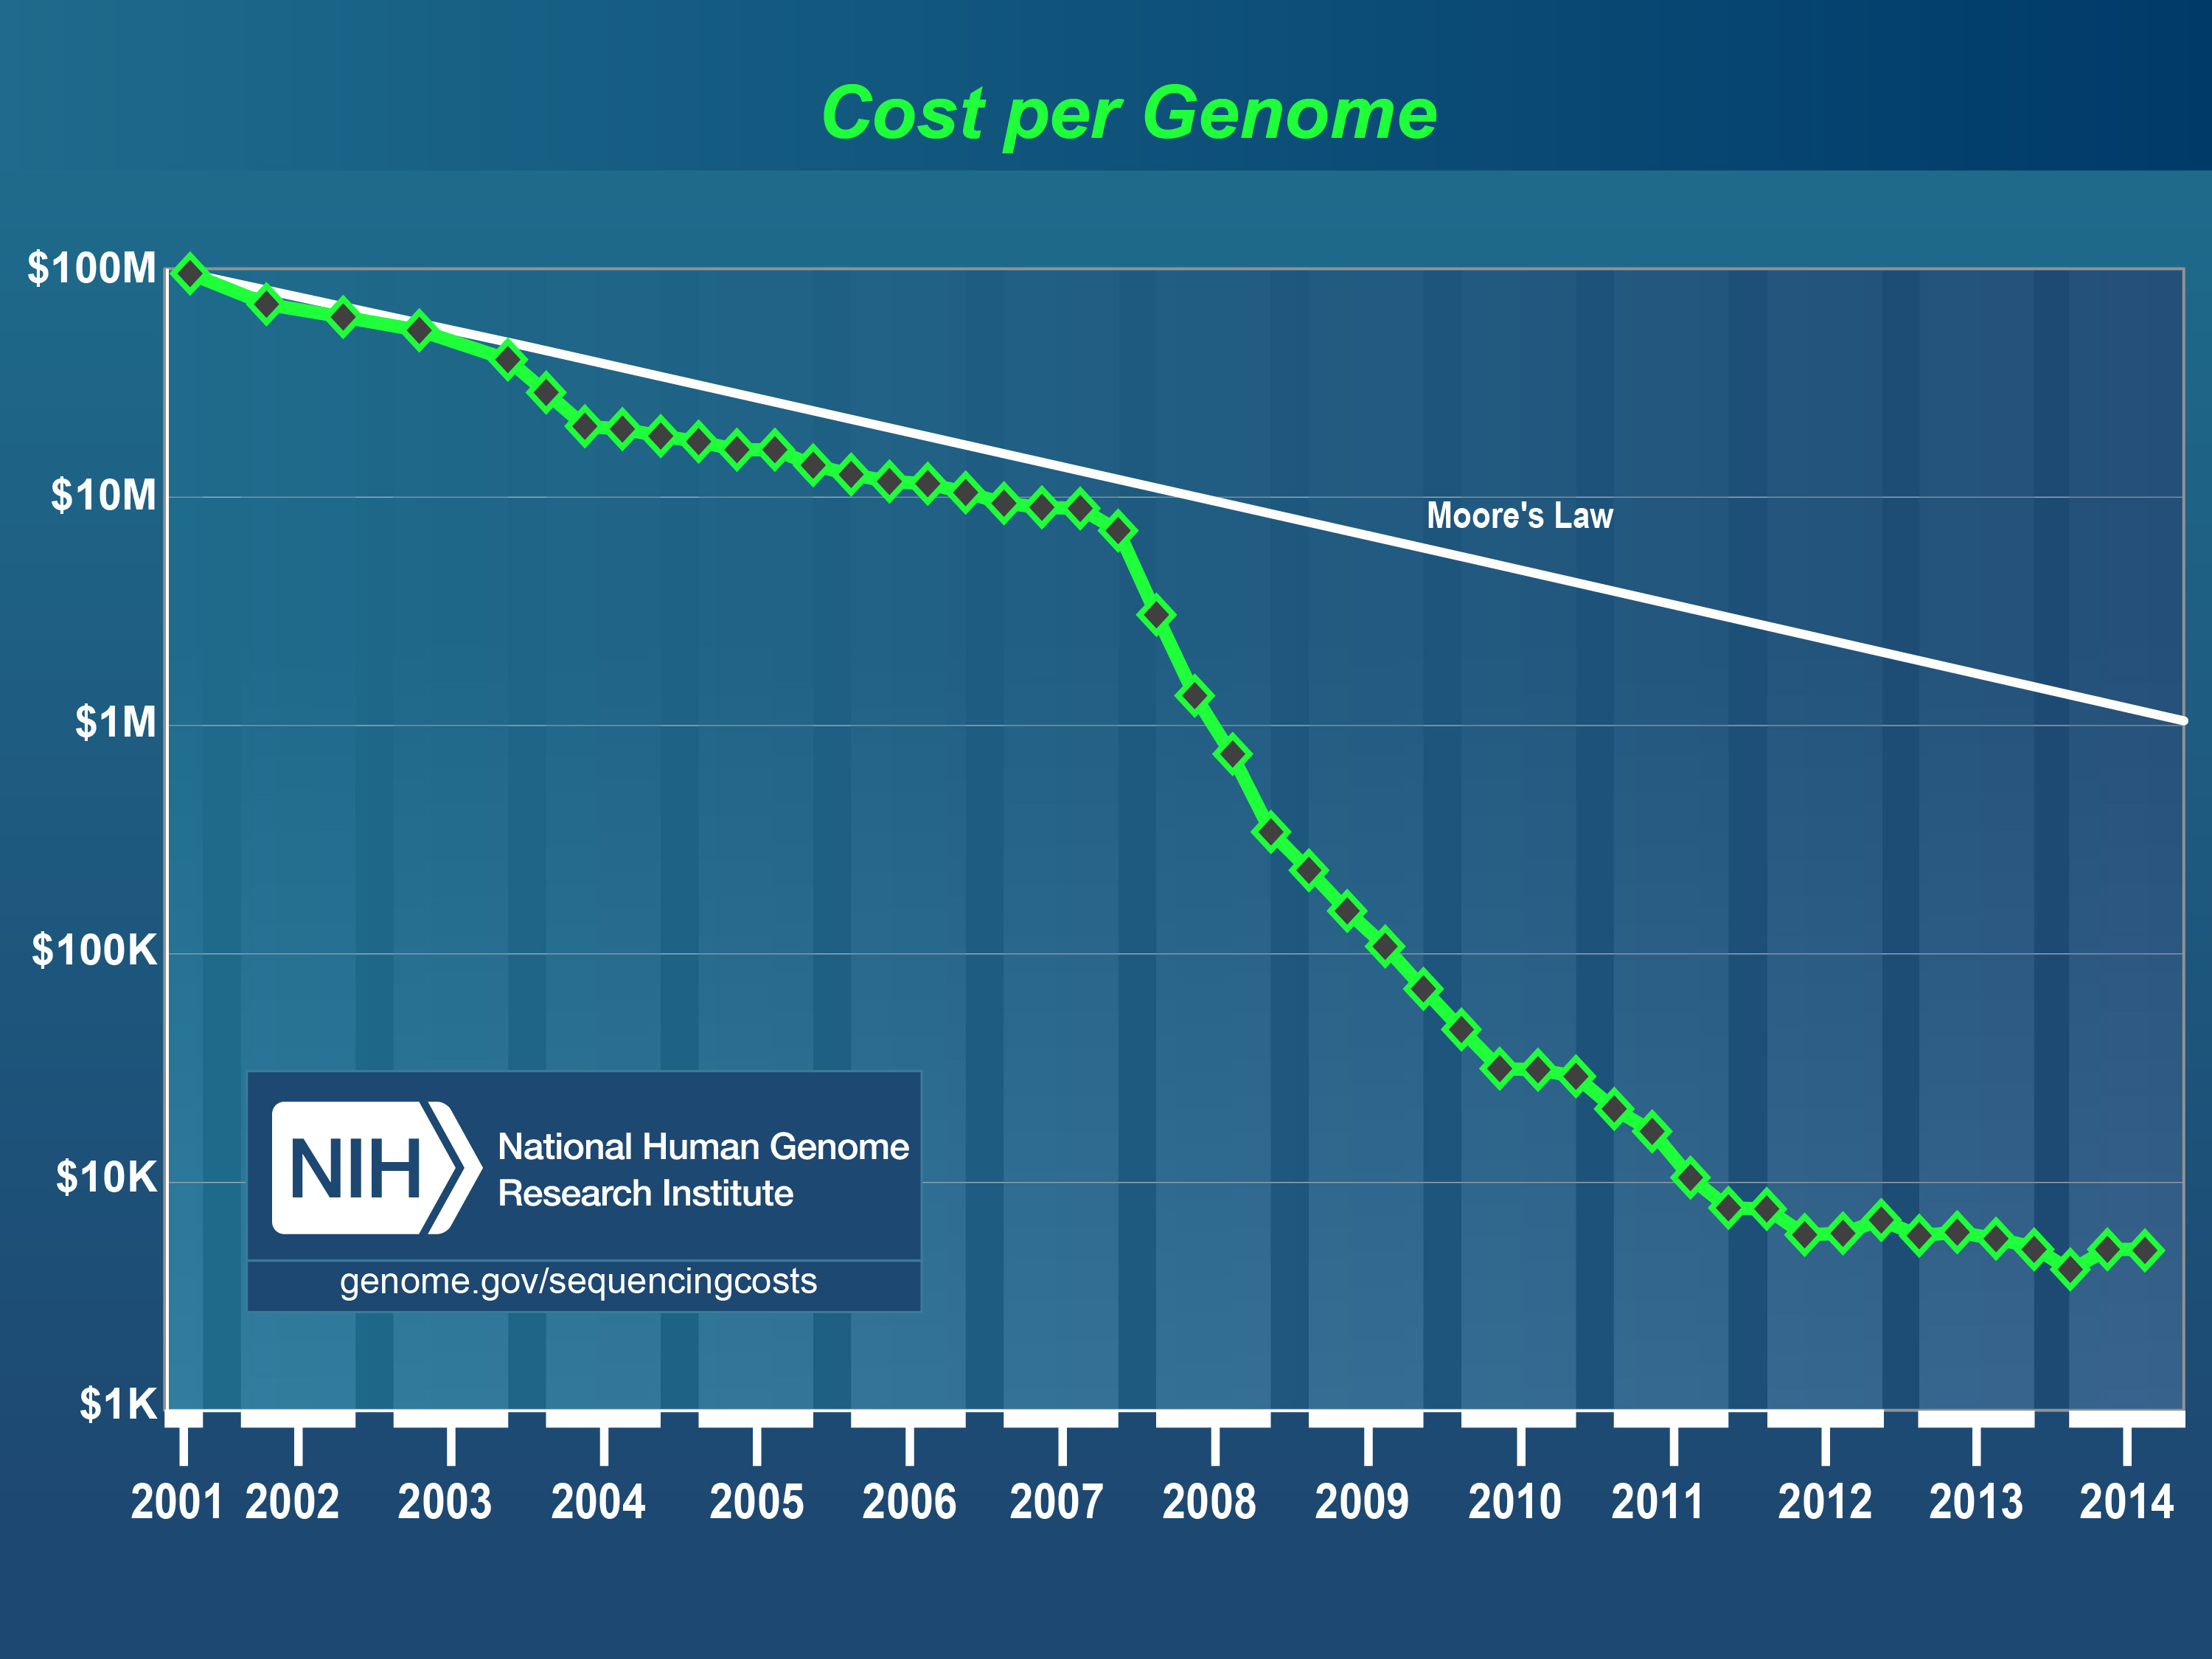
\includegraphics[width=\textwidth,height=\textheight,keepaspectratio]{cost_genome}
\caption{Evolutie van de prijs om een genoom te sequencen sinds 2001}
\label{sequencing_cost}
\end{figure}

\section{GEMINI}

Deze thesis bevat ook een case study over de opportuniteiten voor NoSQL-technologie\"en in de genoomanalysewereld. Op vraag van Janssens Pharmaceutica is het onderwerp hiervan de genoomanalysetool GEMINI (van GEnome MINIng): een software-framework voor flexibele analyse van genetische variaties in grote datasets van genomen, ontwikkeld aan de University of Utah \cite{10.1371/journal.pcbi.1003153}. GEMINI vertrekt daarbij van VCF (Variant Call Format) tekst-bestanden, laadt deze in in een database, voegt allerlei annotaties toe met bijkomende informatie van enkele vermaarde onderzoeksinstituten en biedt dan de mogelijkheid queries uit te voeren op deze databank. De huidige operationele versie van GEMINI draait op de eenvoudige SQL-databank SQLite, maar deze laat op gebied van schaalbaarheid en performantie te wensen over. De gewenste schaalbaarheid ligt in 2 dimensies: enerzijds het aantal genetische \textit{variants} in de dataset, d.w.z. stukken van genen zoals deze in het genoomsequencingproces waargenomen worden, en het aantal proefpersonen of \textit{samples} wier DNA in de dataset geanalyseerd wordt. Bij toenemend 
%TODO getal!
aantal samples of variants duurt zowel het inladen van de genoomdata in de databank voor als het queryen tijdens effectief gebruik te lang om gebruiksvriendelijk te zijn. Het inladen van de genoomdata uit VCF-files is, enigszins contra-intu\"itief, geen eenmalige of zeldzame operatie: de huidige productieversie van GEMINI laat niet toe om na het inladen nog samples of variants toe te voegen, met als gevolg dat bij elke iteratie van een genetisch of biologisch experiment die nieuwe informatie oplevert, de volledige dataset opnieuw ingeladen dient te worden. Ook het incrementeel kunnen toevoegen van variants en samples aan de gegevensset is dus een aandachtspunt bij het onderzoek naar mogelijke verbeteringen voor GEMINI.\\
Een eerste oplossing om de performantie te verhogen was om over te schakelen op PostgreSQL, en hiervan is intussen al met succes een eerste versie ge\"implementeerd. Het resultaat is een verhoging van de querysnelheden van 5 tot 20x, zonder verregaande optimalisaties. De verwachtingen zijn echter ook hier dat PostgreSQL op langere termijn niet zal kunnen schalen naar datasets van (honderd)duizenden genomen.\\
Naar de toekomst toe is het dus noodzakelijk uit kijken naar andere technologie\"en en types databanken om GEMINI ook bruikbaar te maken voor grootschaligere experimenten.

\section{Oplossing, contributies,...}

{\color{red} TODO}




\chapter{Achtergrond genoomanalyse}
\label{dna_dummies}

Omdat deze thesis binnen het vakgebied van de genoomanalyse ligt, volgt in dit hoofdstuk een beknopte inleiding in de wereld van DNA, genomen, genen en aanverwanten, met speciale aandacht voor het DNA van de mens.\\

\section{Biologische achtergrond}
\label{bio_intro}

Desoxyribonucle\"inezuur, kortweg \textbf{DNA}, is de chemische stof die als belangrijkste drager van erfelijke informatie dient in alle levende wezens. DNA bestaat uit twee spiraalvormige, rond elkaar gewikkelde strengen, ook gekend als een dubbele helix. Die twee strengen zijn elk lange ketens van chemische bouwblokken, de nucleotiden, die op hun beurt elk opgebouwd zijn uit 3 delen: een fosfaatgroep, een suikergroep en \'e\'en van 4 mogelijke \textbf{nucleotidebasen}. De 4 nucleotidebasen zijn adenine (A), thymine (T), guanine (G) en cytosine (C). De twee strengen zijn aan elkaar gekoppeld door paren van die basen. Er komen slechts 2 verschillende baseparen voor: AT en GC \cite{genome_gov} \cite{nature_scitable}.\\

Het \textbf{genoom} duidt op de volledige set DNA van een organisme. Het menselijk genoom bestaat uit 3 miljard baseparen. Het grootste deel van DNA bevindt zich in lichaamscellen in de vorm van \textbf{chromosomen}. Menselijke cellen bijvoorbeeld tellen 46 chromosomen, die in 23 paren voorkomen.\\
\textbf{Genen} liggen op de chromosomen en bestaan uit \'e\'en of meerdere DNA-sequenties die de informatie encoderen voor de productie van \'e\'en of meerdere prote\"inen. De deeltjes binnen een gen die effectief die informatie encoderen, heten \textbf{exonen}; de exonen uit alle genen samen worden aangeduid met de term \textbf{exoom} en zijn goed voor ongeveer 1.5\% van het totale DNA \cite{broad_exome}.\\
Genen kunnen verschillende invullingen hebben: sommige genen hebben verschillende vormen die op dezelfde positie op het chromosoom liggen, \textbf{allelen} genaamd. Organismen zoals de mens hebben voor elk gen 2 allelen, \'e\'en overge\"erfd van elke ouder. Zulke organismen worden ook \textbf{diplo\"ide} genoemd. Zijn die twee allelen gelijk, dan is het organisme \textbf{homozygoot} voor het gen in kwestie, anders is het \textbf{heterozygoot}.\\
Het \textbf{genotype} is de specifieke combinatie van allelen die samen het DNA van \'e\'en individueel organisme vormen, m.a.w. de chemische invulling van het DNA. Daartegenover staat het \textbf{fenotype}, dat duidt op de waarneembare fysieke eigenschappen van een levend wezen. Dat kunnen zeer uiteenlopende eigenschappen zijn, gaande van haar- en oogkleur tot het al dan niet lijden aan een bepaalde erfelijke aandoening.\\

Een laatste essentieel biologisch concept is een \textbf{variant} of \textit{single-nucleotide polymorphism} (kortweg SNP of \textit{snip}). Dit zijn korte sequenties DNA die tussen verschillende individuen in een populatie slechts op 1 basepaar verschillen \cite{alberts2007molecular}. In populaties kan voor een variant een referentie en een alternatief allel geobserveerd worden. Diplo\"ide organismen kunnen dus ofwel:
\begin{itemize}
\item Homozygoot voor het referentie allel zijn, wanneer het genotype bestaat uit 2x het referentie-allel.
\item Homozygoot voor het alternatief allel zijn, wanneer het genotype bestaat uit 2x het alternatieve allel.
\item Heterozygoot zijn, wanneer het genotype bestaat uit 1x het referentie-allel en 1x het alternatieve allel.
\end{itemize}
\begin{figure}[!hb]
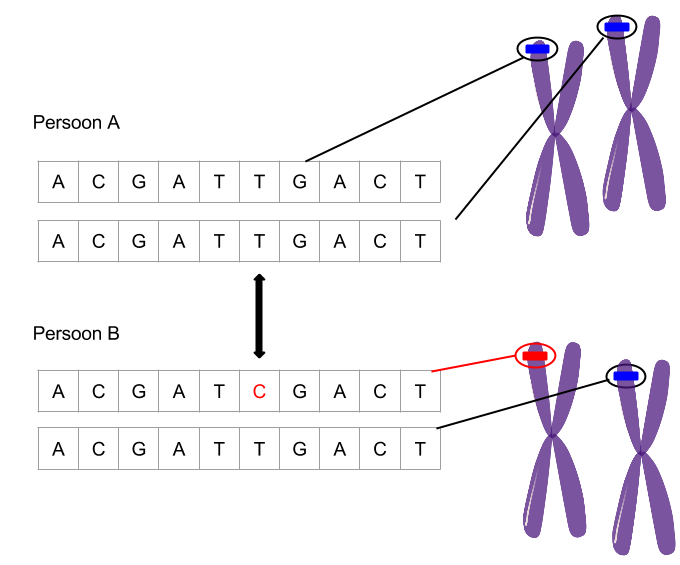
\includegraphics[scale=0.5,keepaspectratio]{chrom_schema}
\caption{Een sequentie uit het DNA van 2 personen. De sequentie ligt op dezelfde locatie op het chromosoom bij beide personen, maar verschilt 1 nucleotide tussen de twee personen. De sequentie is dus een \textit{single nucleotide polymorphism} of \textit{variant}. Beide personen hebben ook twee allelen voor de variant. Persoon A is homozygoot, persoon B heterozygoot \cite{chrom_clipart}.}
\label{chrom_schema}
\end{figure}
Variants zijn zeer belangrijk voor analyse van erfelijke aandoeningen: een nauwe overerving van zowel bepaalde variants als een bepaald fenotype kan de mogelijke locatie van een gen dat een aandoening veroorzaakt reduceren tot een regio op een chromosoom van slechts enkele gensequenties. Die kunnen dan nader onderzocht worden op hun structuur en functie om te bepalen welk gen verantwoordelijk is voor het gemuteerde fenotype. Relevante vragen voor biologen zijn dus welke variants voorkomen bij alle (of veel) individuen met eenzelfde fenotype, en nadien welke variants allemaal in dezelfde regio liggen op een chromosoom. Zoals later (zie \ref{gemini_beschrijving}) uitgebreid aan bod komt, biedt GEMINI ook queries om dit soort vragen te beantwoorden.\\
Figuur \ref{chrom_schema} toont een voorbeeld van de bovenstaande concepten.\\

\section{DNA sequencing}

\textbf{DNA sequencing} is het bepalen van de exacte sequentie van nucleotidebasen in een streng DNA. De vandaag meest gebruikte sequencingmethode genereert reads van 125 opeenvolgende nucleotiden, en miljarden reads tegelijkertijd. Om de segmenten horende in \'e\'en langer stuk DNA aan elkaar te kunnen linken, is het nodig vele overlappende segmenten te lezen, die vervolgens met elkaar gealigneerd worden. Elke nucleotide moet dus meerdere keren gelezen worden om een goede accuraatheid van het uiteindelijke resultaat te bekomen. De \textbf{depth} van een nucleotide, of bij uitbreiding een groter stuk DNA, is het aantal keren dat een nucleotide gelezen werd tijdens het sequencingproces. De \textbf{coverage} is de gemiddelde depth over de hele DNA-streng die gesequenced werd en dus een maat voor de resolutie en nauwkeurigheid van het sequencingproces. De uiteindelijke sequencedata worden vaak opgeslagen in SAM-files (of BAM, het binaire equivalent) en het is op basis hiervan dat \textbf{variant calling} gebeurt: het bepalen welk genotype een proefpersoon precies heeft voor een variant.\\
De resultaten van het variant-callingproces worden opgeslagen in \textbf{VCF}-bestanden (Variant Call Format). Het VCF-formaat bevat naast meta-informatie een lijn voor elke geobserveerde variant, met daarin optioneel informatie over het genotype van \'e\'en of meerdere proefpersonen.\\
In onderzoek naar het DNA van proefpersonen is ook nog andere informatie van tel dan enkel hun genotypes: gegevens als het geslacht of fenotype van proefpersonen kunnen uiterst relevant zijn voor onderzoek naar bijvoorbeeld genetische ziektes. In experimenten die het DNA van meerdere proefpersonen analyseren, is het ook bijzonder interessant de onderlinge verwantschappen tussen de proefpersonen te kennen. Samen met de genotype-informatie is het dan mogelijk erfelijkheidspatronen in de genoomdata te bestuderen. Informatie over de proefpersonen zit niet in VCF-files, maar kan gespecifieerd worden in pedigree-files (\textbf{PED}-files).\\\\

\section{Voorbeeldvraagstukken genoomanalyse}

Deze sectie schetst kort een voorbeeld van de soort analyses die biologen maken met behulp van tools zoals GEMINI, en de extra informatie die ze hiervoor nodig hebben.\\
Biologen kunnen bijvoorbeeld ge\"interesseerd zijn in:
\begin{itemize}
\item Variants die gelinkt zijn met bepaalde aandoeningen. Van sommige variants is hun correlatie met erfelijke aandoeningen reeds bekend en die informatie kan in annotaties samengevat worden. Zo kent GEMINI bijvoorbeeld de volgende annotaties:
\begin{itemize}
\item \texttt{is\_somatic}: variants kunnen somatisch verworven mutaties zijn. Dit zijn mutaties die na de bevruchting optreden en later tot kanker of andere ziekten kunnen leiden.
\item \texttt{clinvar\_disease\_name}: de naam van de aandoening waarvoor de variant relevant is.
\end{itemize}
\item Variants die vaak voorkomen in specifieke populaties. Zo kent GEMINI bijvoorbeeld de \texttt{aaf\_1kg\_afr}-annotatie, die de allel-frequentie (de frequentie waarmee een allel in een populatie voorkomt) in het genotype van proefpersonen van Afrikaanse origine uit het 1000 Genomes project voorstelt.
\item Variants die op een bepaalde positie in het DNA liggen. Zoals aangehaald in \ref{bio_intro}, proberen biologen de oorzaak van aandoeningen te beperken tot een zo klein mogelijke regio in het DNA. Daarvoor is het nuttig te kunnen zoeken naar variants die op een specifiek chromosoom binnen een bepaald bereik van startposities liggen.
\item Variants waarvoor bepaalde proefpersonen een bepaald genotype hebben. Zo kan het interessant zijn te zoeken naar variants die voorkomen in het DNA van proefpersonen met een aandoening (i.e. waarvoor die homozygoot zijn voor het referentie-allel), terwijl ze niet voorkomen in het DNA van gezonde personen. Dit kan kleinschalig gebeuren, door bijvoorbeeld de genotypes van een kind en zijn ouders te vergelijken, of op grotere schaal door een volledige populatie van proefpersonen te bestuderen.
\end{itemize}
\chapter{Achtergrond datastores}
\label{datastores_intro}

Sinds de jaren '70 zijn zogenaamde \textit{relational database management systems} (kortweg RDBMS) de voornaamste technologie voor de grootschalige opslag van gegevens. Ze zijn gestoeld op 2 belangrijke principes, namelijk het relationele datamodel \cite{codd1970relational} en de gestructureerde querytaal SEQUEL, beter gekend als SQL \cite{chamberlin1974sequel}. De architectuur van vele RDBMS is nog steeds gebaseerd op de eerste implementatie van een dergelijk systeem, namelijk het IBM onderzoeksproject System R \cite{blasgen1981system}, ook uit halverwege de jaren '70 \cite{Stonebraker:2007:EAE:1325851.1325981}. System R is uiteraard ontworpen voor destijds relevante hardwarekarakteristieken en productvereisten: business data processing via een command line interface, en dit op computersystemen met trage processoren, kleine werk- en schijfgeheugens maar relatief grote bandbreedte tussen de schijfopslag en het werkgeheugen. Dit leidde tot een aantal architecturale features die nog steeds terug te vinden zijn in hedendaagse RDBMS:
\begin{itemize}
\item Disk-geori\"enteerde opslag- en indexstructuren
\item Multithreading om latency op te vangen
\item Concurrency-controlemechanismen op basis van locking
\item Log-gebaseerd herstel van fouten
\end{itemize} 
Ondanks gigantische technologische vooruitgang op gebied van hardware en sterk gediversifieerde gebruiksscenario's, is er sinds hun ontstaan 40 jaar geleden weinig drastisch veranderd aan het concept van de RDBMS en zijn deze systemen de werkpaarden van de industrie geworden op het vlak van dataopslag.\\

Beginnende in de jaren 2000 groeide in de IT-wereld dan ook het besef dat de rigide \textit{one size fits all}-aanpak van RDBMS voor vele moderne toepassingen achterhaald dreigde te geraken. Met grote opkomende spelers uit de web-industrie zoals Google, Amazon en Facebook aan het roer leidde dit tot de opkomst van de NoSQL-beweging. NoSQL staat, in tegenstelling tot wat de naam doet vermoeden, voor \textit{Not only SQL} en omvat een waaier van uiteenlopende alternatieve gegevensopslagsystemen die elk in bepaalde specifieke opzichten meerwaarde trachten te bieden ten opzichte van het klassieke relationele systemen. In tegenstelling tot de 'Zwitsers zakmes'-aanpak van RDMBS, leggen ze zich toe op zeer gespecialiseerde toepassingsdomeinen en proberen daarin relationele systemen te overtreffen. Vaak betekent dit dat NoSQL systemen vele voor hun doel onnodig geachte features van SQL systemen achterwege laten, of afzwakken. Een goed voorbeeld hiervan zijn de ACID-eigenschappen uit het relationele model die in vele NoSQL-systemen gereduceerd zijn tot zogenaamde BASE-eigenschappen (op het verschil tussen beide komt sectie \ref{consistentie} nog uitgebreid terug).

De reden waarom web-spelers overstapten op NoSQL-systemen of er zelf ontwierpen, is voornamelijk dat deze geschikter zijn voor de enorme hoeveelheden data die dergelijke bedrijven sinds de opkomst van Web 2.0 moeten verwerken. NoSQL-systemen staan er om bekend horizontaal en incrementeel te schalen naar gigantische datasets: door eenvoudigweg servers toe te voegen aan de cluster onder de databank, en niet door bestaande servers up te graden (i.e. verticaal schalen), kan een cluster vlot meegroeien met de dataset. Bovendien draaien NoSQL-systemen doorgaans op goedkope commodity hardware, dus standaard servers, in plaats van dure gespecialiseerde databankservers. Goedkope doordeweekse servers laten toe om zowel kost- als energie-effici\"enter redundantie en dus ook fouttolerantie in te bouwen en zo de zeer hoge vereiste beschikbaarheid te garanderen \cite{barroso2003web}. NoSQL-systemen zijn bijgevolg grootschalige, gedistribueerde systemen, met bijhorende mechanismen om data ten eerste op te splitsen en te verspreiden (ook: partitioneren of sharden) en ten tweede te repliceren over de cluster. Replicatie heeft meerdere doelen: verhoogde bedrijfszekerheid, load balancing en verhoogde doorvoer in lees-intensieve toepassingen.

\section{Concepten}

Deze sectie belicht de belangrijkste begrippen in verband met NoSQL-databanken en contrasteert waar nodig met gelijkaardige concepten in het klassieke traditionele model.

\subsection{Partitionering}

Gezien de grote datahoeveelheden en gedistribueerde setting van NoSQL is het een noodzaak data in de databank te verspreiden. Er bestaan meerdere strategie\"en om de entries in een databank (dit kunnen rijen, documenten, simpele values,\ldots zijn) over de nodes in een cluster te verdelen. Ten eerste is er het onderscheid tussen horizontaal en verticaal partitioneren: bij horizontaal schalen, ook sharding genoemd, wordt een entry niet gefragmenteerd, maar in zijn geheel toegewezen aan een node, op basis van een op de entry gedefinieerde key. De meeste NoSQL datastores implementeren een versie van horizontaal partitioneren. Verticaal partitioneren stamt uit het relationele model, en betekent het splitsen van grote tabellen in meerdere kleinere tabellen.\\
Binnen het horizontaal partitioneren bestaan 2 voorname methodes \cite{grolinger2013data}:
\begin{itemize}
\item \textit{Range partitioning:} elke server is verantwoordelijk voor een bepaald bereik van key-waarden. Deze methode leent zich uitstekend tot het verwerken van range queries, gezien opeenvolgende keys vaak op eenzelfde node zullen liggen. Er is echter ook een belangrijk nadeel met deze aanpak verbonden: ze kan leiden tot load-balanceringsproblemen en \textit{hot spots}. Wanneer een applicatie bijvoorbeeld de gegevens in volgorde van hun key-waarden verwerkt, zal de werklast steeds bij dezelfde servers geconcentreerd liggen. Een ander nadeel is dat een centrale routing server de mapping van de ranges van keys naar nodes moet bijhouden, die dan client requests naar de juiste nodes door kan sturen. Dit introduceert een mogelijke flessenhals in het systeem.
\item \textit{Consistent hashing:} zoals de naam doet vermoeden, gebeurt de partitie in dit geval op basis van een hash van de key van entries. De output van de hash-functie wordt als een ring beschouwd en alle nodes krijgen een willekeurige waarde of positie toegewezen op deze ring. Een entry wordt dan toegewezen door via de hash van zijn key zijn positie in de ring te bepalen en vervolgens de ring klokwijs te bewandelen tot de eerste node met positie groter dan de positie van de entry. Het voordeel van consistent hashing is dat de positie van een object zeer snel berekend kan worden en dat hier geen centraal bewaarde mapping voor nodig is. Bovendien is het toevoegen van nodes zeer eenvoudig: enkel de buren van een nieuwe node op de ring merken dit, waardoor weinig entries verplaatst moeten worden. Een belangrijk nadeel is dat consistent hashing range queries bemoeilijkt, gezien opeenvolgende entries nu verspreid kunnen liggen over verschillende nodes.\\
Een techniek die vaak gepaard gaat met consistent hashing is het gebruik van \textit{virtual nodes} om load-balancing te verbeteren: elke fysieke node in de cluster krijgt meerdere posities toegewezen op de ring, en is zo verantwoordelijk voor meerdere virtuele nodes. Dit zorgt voor een betere verdeling van de entries over de nodes, gezien entries niet per se uniform over de ring verdeeld liggen. Bovendien moeten niet alle fysieke nodes verantwoordelijk zijn voor evenveel virtuele nodes: het systeem kan meer virtuele nodes toewijzen aan performantere fysieke nodes en zo rekening houden met heterogeniteit in de fysieke infrastructuur. Bovendien zal, bij het falen van een fysieke node, zijn opgeslagen last eerlijk verspreid worden tussen de overgebleven fysieke nodes. Omgekeerd zal een nieuwe node wanneer hij toetreedt tot de cluster van alle andere fysieke nodes ongeveer evenveel last overnemen  \cite{grolinger2013data}\cite{decandia2007dynamo}.
\end{itemize}  

\subsection{Consistentie}
\label{consistentie}

Consistentie van database-transacties betekent dat transacties de databank in een consistente staat achterlaten: alle data die een applicatie kan zien, is een consistente snapshot van de databank \cite{ports2010transactional}. Traditionele RDBMS bieden vaak transacties met de zogenaamde ACID-eigenschappen \cite{haerder1983principles}:
\begin{itemize}
\item \textbf{Atomicity:} Elke transactie gebeurt ofwel volledig, ofwel helemaal niet.
\item \textbf{Consistency:} Elke transactie laat de databank in consistente staat achter.
\item \textbf{Isolation:} Elke transactie verloopt volledig ge\"isoleerd van elke andere transactie en be\"invloedt deze dus op geen enkele manier.
\item \textbf{Durability:} Eens voltrokken, blijft elke transactie duurzaam bewaard in de databank, ook in het geval van stroomonderbrekingen, crashes of fouten.
\end{itemize}

Zoals Eric Brewer stelde in zijn bekende CAP-theorema \cite{brewer2000towards}, is het in een gedistribueerd systeem niet eenvoudig zowel consistentie, availability als tolerantie voor partities te bereiken en zijn 2 van deze 3 eigenschappen het hoogst haalbare\footnote{Brewer kwam hier zelf 12 jaar later op terug, stellende dat mits goede omgang met partities het toch mogelijk is een trade-off van alle drie te bereiken \cite{brewer2012cap}.}.
Ook in NoSQL-systemen, die vaak gedistribueerd van aard zijn, is het garanderen van consistentie geen triviale opgave. Afhankelijk van de gehanteerde schrijfstrategie is het mogelijk dat verschillende knopen in de cluster verschillende versies van data zien, als updates nog niet in de volledige cluster doorgekomen zijn. Daarom is er het onderscheid tussen strikte en uiteindelijke ("\textit{eventual}") consistentie: strikte consistentie is de gekende vorm waarin updates onmiddellijk zichtbaar zijn op alle nodes in de cluster, en dus ook naar bovenliggende applicaties toe. In het geval van uiteindelijke consistentie garandeert het systeem enkel dat na verloop van tijd alle nodes in de cluster dezelfde, up-to-date versie van de data zullen zien. NoSQL-systemen bieden dan ook vaak de BASE-eigenschappen, een zwakkere versie van de ACID-garanties:
\begin{itemize}
\item \textbf{Basically available:} Het systeem is onder quasi alle omstandigheden beschikbaar.
\item \textbf{Soft state:} Het systeem verkeert niet altijd in een consistente staat
\item \textbf{Eventually consistent:} Na verloop van tijd zal het systeem in een gekende staat verkeren.
\end{itemize}

Vele NoSQL-systemen stellen de gebruiker echter niet voor een voldongen feit bij de keuze tussen strikte en uiteindelijke consistentie: dankzij zogenaamde \textit{quora} kan de gebruiker zelf configureren welke consistentie het systeem levert. Door lees- en schrijfquora in te stellen, kan de gebruiker tunen hoeveel replica's respectievelijk moeten returnen bij een schrijfopdracht, en het welslagen van een schrijfopdracht moeten bevestigen. Op deze manier kan de gebruiker zelf een trade-off maken tussen snel lezen, schrijven en de behaalde consistentie. Bovendien zal de gebruiker, wanneer de som van het lees- en schrijfquorum groter is dan de replicatiefactor van de cluster, steeds de meest recente versie van gegevens zien, wat hetzelfde betekent als onmiddellijke, strikte consistentie.

\subsection{Storage layout}
\label{storage_layout}
Ook op het gebied van hoe ze gegevens zowel op schijf als in het geheugen opslaan, verschillen NoSQL-systemen van elkaar. Sommigen hanteren de gebalanceeerde B-bomen die ook vele RDBM-systemen gebruiken. Anderen, in navolging van Google Bigtable, doen beroep op zogenaamde \textit{log-structured merge trees}. In deze strategie worden updates niet onmiddellijk naar schijf geschreven: de data wordt in werkgeheugen aangepast en de update wordt op schijf gelogd. Wanneer er genoeg updates in geheugen gebeurd zijn, worden deze allemaal tegelijkertijd naar schijf geschreven. Dit kan sequentieel gebeuren, en vermijdt zo vele random writes, wat de schrijfdoorvoer uiteraard ten goede komt. 


\section{NoSQL-klassen}

NoSQL databanken zijn er in verschillende soorten en kunnen op basis van hun datamodel in een aantal categorie\"en onderverdeeld worden:

\begin{itemize}
\item \textbf{Key-Value stores} zijn vergelijkbaar met dictionaries en mappen unieke keys op values. Deze values zijn voor de databank volledig betekenisloze byte-arrays en de enige manier om ze op te vragen, is via de bijhoren key. Voor zeer eenvoudige toepassingen resulteert dit in hoge lees- en schrijf-throughput, maar meer geavanceerde features zoals indexing, queries, en het modelleren van relaties binnen de data zijn hierdoor niet mogelijk\cite{hecht2011nosql}\cite{grolinger2013data}.

\item \textbf{Columnar stores}
\label{Bigtable} zijn gebaseerd op het datamodel dat Google's Bigtable heeft ge\"introduceerd en slaan data op in een spaarse, gedistribueerde, persistente en multidimensionele gesorteerde map\cite{chang2008bigtable}. In het geval van Bigtable zijn dit drie dimensies: row key, column key en een timestamp. Bigtable is voorzien op de enorme hoeveelheden data die Google op dagelijkse basis verwerkt en de hiervan afgeleide columnar stores staan dan ook bekend om hun uitstekende schaalbaarheid. De goede schaalbaarheid en fouttolerantie van Bigtable is ook deels toe te schrijven aan het onderliggende gedistribueerde file systeem, Google File System \cite{ghemawat2003google}. Andere innovaties uit Bigtable zijn onder andere het gebruik van log-structured merge trees (zie \ref{storage_layout}) en Bloom filters: een effici\"ent probabilistische mechanisme om te voorspellen of een object in een verzameling zit (in dit geval, of een key in een tabel ligt, wat het aantal nodeloze table scans beduidend kan inperken) \cite{mullin1983second}.\\
Omdat net als in Key-Value stores het systeem hier de opgeslagen data niet interpreteert, is het modelleren van relaties niet op een effici\"ente manier mogelijk. Dit wordt overgelaten aan de bovenliggende applicatie \cite{hecht2011nosql}.

\item \textbf{Document stores} bewaren data als key-value paren en encapsuleren deze in documenten. Values kunnen van een brede waaier aan types zijn, zoals geneste documenten, lijsten of scalars. De namen van attributen kunnen dynamisch gespecifieerd worden tijdens runtime en moeten geen vooraf vastgelegd schema volgen\cite{cattell2011scalable}. Dit is geschikt voor het modelleren van ingewikkelde datastructuren. Vele document stores gebruiken het JSON-bestandsformaa (of een daarvan afgeleide vorm). In tegenstelling tot columnar stores, zijn de waarden in documenten niet betekenisloos voor het document store systeem en het is dus mogelijk hier indexen op te defini\"eren en queries op uit te voeren \cite{hecht2011nosql}.

\item \textbf{Graph databases:} zoals de naam doet vermoeden, stammen ze uit grafentheorie en maken ze gebruik van grafen als datamodel. Ze zijn uitermate geschikt om sterk verweven data te beheren, van bronnen zoals sociale netwerken of location based services. Hiervoor doen ze beroep op effici\"ente mechanismen om grafen te doorlopen waar andere systemen kostelijke operaties als recursieve joins gebruiken\cite{hecht2011nosql}.

\end{itemize}

De term NewSQL slaat op een verzameling systemen die ambi\"eren het klassieke relationele datamodel te combineren met de schaalbaarheid, distributie en fouttolerantie van NoSQL systemn. Hoewel ze allen de gebruiker het relationele model en SQL-achtige query mogelijkheden bieden, verschillen NewSQL stores onderling grondig, afhankelijk van de onderliggende architectuur. Zo zijn er onder meer systemen die gebouwd zijn bovenop bestaande NoSQL databanken, en andere die alle data in main memory opslaan.\cite{grolinger2013data}

\section{NoSQL: vergelijkende studie}
\label{nosql_survey}

Op de vraag of NoSQL en NewSQl-systemen al dan niet geschikt zijn om het genoomanalyseproces schaalbaarder te maken, bestaat geen eenvoudig antwoord. Gezien de grote diversiteit in de beschikbare gegevensopslagsystemen, zullen sommige systemen onvermijdelijk beter geschikt zijn dan andere, of beter geschikt voor andere aspecten van de genoom-analyse pipeline. Een vergelijkende studie van NoSQL- en NewSQL-systemen dringt zich dus op. Deze sectie bekijkt 6 systemen in meer detail en licht toe hoe ze van pas zouden kunnen komen in de genoomanalyse.

\subsection{Methodologie}

Omwille van het enorme aanbod aan NoSQL en NewSQL systemen was een exhaustieve studie niet haalbaar. Deze vergelijkende studie behandelt de populairste datastores in een aantal relevante categorie\"en, namelijk document stores, columnar stores en NewSQL stores. Key-value stores en graph databases komen niet aan bod, aangezien hun datamodellen niet geschikt zijn voor de toepassing in kwestie. De uiteindelijke selectie werd gemaakt volgens criteria vergelijkbaar met die in \cite{grolinger2013data}, met de ranking van DB-Engine Ranking \cite{db_engine_rank} als maat voor de populariteit.\\

\begin{landscape}
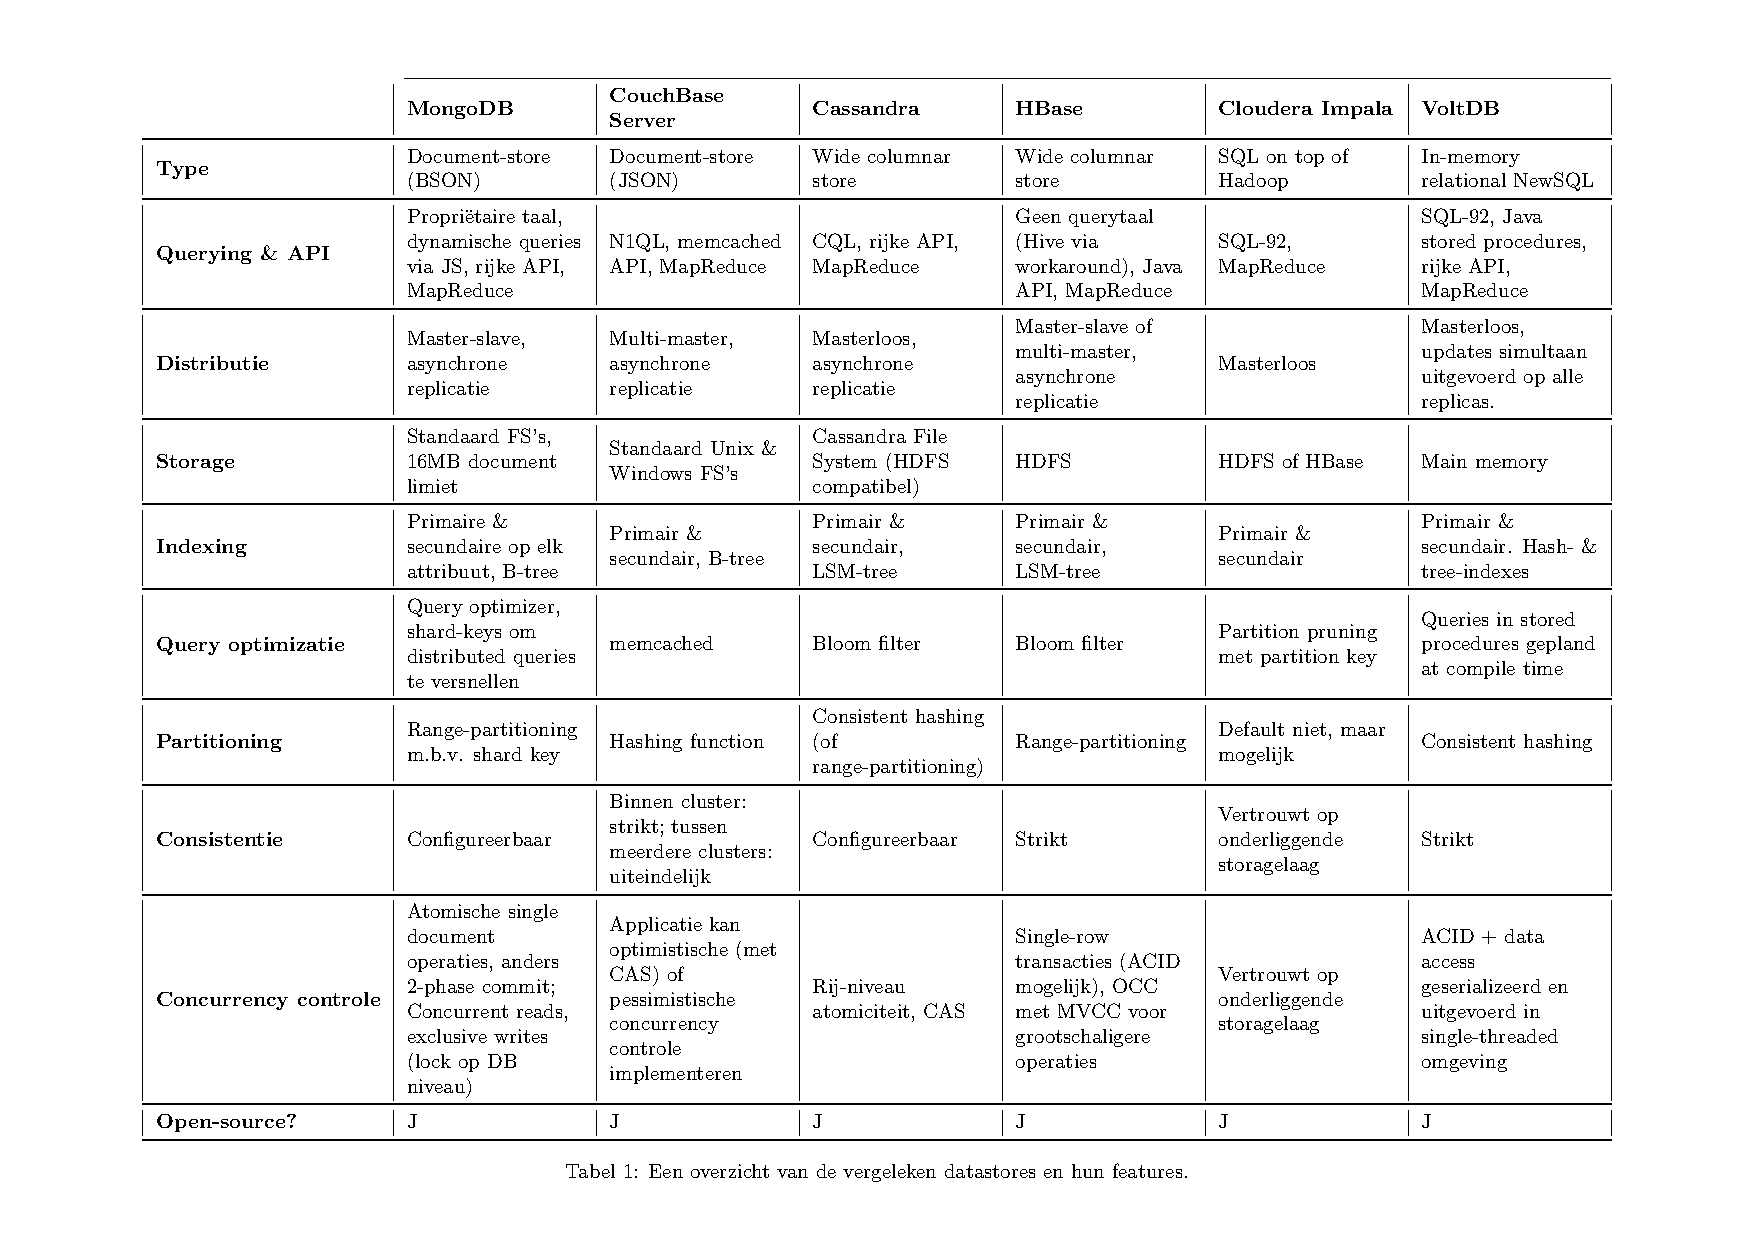
\includepdf[angle=90]{NoSQL_table_nl.pdf}
\label{survey_tabel}
\end{landscape}

Deze ranglijst tracht populariteit te meten op basis van enkele parameters, zoals aantal vermeldingen op websites, algemene interesses volgens Google Trends, frequentie van technische discussies op fora zoals StackOverflow, vacatures i.v.m. de technologie en vermeldingen in professionele profielen op sites zoals LinkedIn. De resulterende selectie bestaat uit de document stores MongoDB en CouchBase Server, wide columnar stores Cassandra en HBase en NewSQL database VoltDB. Er bestaat al een uitbreiding van de DNA sequencing pijplijn die het ExaScience Life Lab gebruikt om MongoDB  databanken als in- en/of uitvoer te gebruiken voor de pijplijn. Dit maakt MongoDB uiteraard nog relevanter. Ten laatste werd ook NewSQL query engine Cloudera Impala in de studie betrokken wegens expliciete interesse van onderzoekers in het eerder vernoemde lab.

\noindent Deze 6 systemen vergeleken we vervolgens op een aantal voor high performance computing relevante eigenschappen zoals indexeringsmechanismen, interfaces naar de gebruiker en API's, distributiestrategie, concurrency controle en consistentiemodel. Tabel \ref{survey_tabel} geeft een overzicht weer van de bestudeerde systemen.

\subsection{Document stores}

\subsubsection{MongoDB}

MongoDB slaat gegevens op in BSON (binary JSON) documenten. Het systeem biedt krachtige ondersteuning voor indices, vooral door de mogelijkheid om secundaire indices van een brede waaier van types te defini\"eren op alle attributen, zoals in het relationele model. Deze indices zijn gebouwd op B-trees \cite{mongodb_indexes}. Om denormalizatie te bevorderen, kunnen documenten geneste documenten en arrays bevatten. Zo zijn joins ook overbodig in de query taal.\\
De bestandsgrootte is beperkt tot 16 MB, om te voorkomen dat \'e\'en enkel document buitensporig veel RAM of bandbreedte opeist. Om grotere bestanden te bewaren, kan het ingebouwde GridFS (dat integenstelling tot wat de naam doet vermoeden, geen volwaardig file system is) automatisch bestanden opsplitsen in kleinere delen en deze delen als aparte documenten bewaren, zonder dat de gebruiker zich hierom moet bekommeren.\\
MongoDB biedt API's in zeer vele programmeertalen en de functionaliteit om het equivalent van SQL \texttt{WHERE}-clausules te defini\"eren als javascript uitdrukkingen. MongoDB vertaalt deze vervolgens naar een eigen, interne en afgeschermde query taal \cite{grolinger2013data}. De query optimizer van MongoDB verwerkt queries en kiest voor elke query een zo effici\"ent mogelijk uitvoeringsplan gegeven de beschikbare indices. Deze plannen worden gecached als er meerdere goede alternatieven zijn en kunnen geherevalueerd worden naarmate de gegevensset in de databank evolueert.\\
Qua consistentie laat MongoDB de keuze tussen uiteindelijke en strikte consistentie. Strikte consistentie is mogelijk door ofwel enkel te lezen van de master node (die de meest up-to-date versie van de data heeft) of na schrijfopdrachten te wachten tot alle replica's bevestigd hebben alvorens verder te gaan. De eerste optie introduceert een bottleneck bij het lezen van data, de tweede verhoogt de latentie van schrijfopdrachten.\\
MongoDB repliceert data asynchroon en partitioneert in ranges: nodes zijn verantwoordelijk voor ranges van keys. Dit zorgt voor snelle range queries, maar kan hotspots en load-balancingproblemen veroorzaken. Dankzij een master-slave struktuur kan MongoDB updates gemakkelijk naar de juiste replica's doorverwijzen.
Op het gebied van concurrency controle biedt MongoDB atomiciteit binnen documenten en reader-writer locks. Bij schrijfopdrachten de databank locken heeft een zware impact op de performantie in scenario's waar veel geschreven moet worden.\\\\
Kortom, MongoDB bewaart BSON-bestanden op een zeer toegankelijke manier met flexibele query- en indexeringsmechanismes. De concurrency- en consistentiemodellen daarentegen vertonen enkele nadelen.

\subsubsection{Couchbase Server}

Couchbase, het resultaat van de fusie tussen CouchDB en Membase, slaat gegevens op in JSON documenten. Het hanteert het memcached protocol om een gedistribueerde cache en is bedoeld voor zeer interactieve toepassingen met hoge vereisten op gebied van latentie \cite{grolinger2013data}\cite{couchbase_about}.
De JSON documenten kunnen genest zijn en kunnen doorzocht worden met een uitgebreide, SQL-achtige taal, N1QL (op het moment van schrijven is dit wel nog steeds een developer preview, uitgebracht in januari 2015) \cite{couchbase_n1ql}.
Net als MongoDB kunnen primaire en secundaire indices gedefinieerd worden en zijn deze gestoeld op B-trees \cite{couchbase_index}.\\
Binnen \'e\'en cluster zijn transacties strikt consistent, maar tussen meerdere clusters slechts uiteindelijk consistent.\\
CouchBase biedt gebruikers de keuze tussen optimistische (m.b.v. compare-and-swap) en pessimistische (m.b.v. 'finegrained locking') concurreny controle.\\\\
Dankzij zijn flexibele datamodel, caching en concurrency controle, past CouchBase goed voor toepassingen die snelle en intensieve interactieve vergen tussen gebruiker en data.

\subsection{Columnar stores}

\subsubsection{Cassandra}

Cassandra werd oorspronkelijk ontwikkeld voor intern gebruik bij Facebook maar is later als Apache opensourceproject publiekelijk beschikbaar gemaakt. Het combineert het columnaire datamodel van Google's Bigtable systeem (zie \ref{Bigtable}) met de architectuur en distributiestrategie van Amazons DynamoDB. Het is gericht op flexibele, quasipermanent beschikbare opslag van zeer grote datasets op goedkope standaardhardware, met daarenboven hoge througput voor schrijfopdrachten zonder effici\"entie bij leesopdrachten op te offeren \cite{borthakur2011apache}.\\
Sinds zijn ontstaan is Cassandra wel op enkele vlakken afgeweken van het BigTable-model \cite{cassandra_then&now}, in die zin dat het nu tabellen en \textit{composite columns} biedt, evenals een eigen query taal, CQL \cite{cassandra_CQL}. CQL vertoont op het gebied van syntax en functionaliteit sterke gelijkenissen met SQL, maar is toch sterk beperkt. Zo biedt het bijvoorbeeld geen \texttt{JOIN}-clausule, en zijn \texttt{WHERE}-clausules aan sterke voorwaarden onderhevig. Cassandra moedigt het samen bewaren van gegevens die samen opgevraagd worden sterk aan en ondersteunt denormalizatie met features zoals collection types.\\
Cassandra heeft indexeringsmechanismes and implementeert deze met log-structured merge trees, met hogere schrijfthroughput als gevolg. Ook biedt Cassandra net als Google Bigtable Bloom filters.\\
Om lineair in het aantal ingeschakelde nodes te kunnen schalen naar zeer grote datasets, opereert Cassandra op een volledig hi\"erarchieloze wijze. Vanuit het perspectief van het CAP-theorema, spitst Cassandra zich toe op availability en partition tolerance, ten koste van onmiddellijke consistentie. Het consistentieniveau kan wel per query door de gebruiker bepaald worden, zoals later verduidelijkt wordt. Hoge beschikbaarheid en tolerantie voor fouten bereikt Cassandra door asynchroon data te repliceren over verschillende nodes, met consistent hashing en virtuele nodes om frequent komen-en-gaan en incrementeel toevoegen van nodes op te vangen. Het aantal replica's kan de gebruiker zelf kiezen. Bovendien voorziet Cassandra ook interdatacenterreplicatie, om zelfs het falen van volledige datacenters op te vangen \cite{decandia2007dynamo} \cite{lakshman2010cassandra} \cite{cassandra_then&now}.\\
Bij lees- en schrijfopdrachten kan de gebruiker een quorum specifi\"eren. Hoewel Cassandra met uiteindelijke consistentie voor het oog ontworpen werd, is onmiddellijke consistentie mits een juiste keuze van de quorum dus ook een optie.\\
Op het gebied van concurrency controle garandeert Cassandra atomiciteit binnen rijen en serializeerbare \textit{lightweight transactions}, eigenlijk compare-and-set functionaliteit, voor grotere operaties.
\\\\
Samengevat biedt Cassandra redelijk flexibele datamodellering met (licht beperkte) query- en indexeringsmechanismen via de CQL-interface. Het sterkste punt is echter dat Cassandra incrementeel schaalt naar enorme datasets, dankzij uitvoerige replicatie- en foutverwerkingsfeatures.

\subsubsection{HBase}

Apache HBase is een opensource datastore gebaseerd op Google Bigtable, die draait bovenop het Hadoop Distributed File System (HDFS) in plaats van het Google File System (GFS).\\
Sinds z'n lancering heeft HBase verschillende secundaire indexeringsmechanismes verworven. Deze zijn ook gebaseerd op LSM trees en daarnaast biedt ook HBase Bloom filters \cite{borthakur2011apache}\cite{hbase_schema}. HBase heeft een Java API, maar zonder SQL-achtige geavanceerde querytaal. Hierbij moet wel opgemerkt worden dat een omweg via Apache Hive, een ander data-opslag en -analyseproject \cite{apache_hive}, en de bijhorende querytaal HiveQL dit probleem kan verhelpen. Dankzij de HDFS-fundering can HBase vlot fungeren als in- en output voor MapReduce taken.\\
HBase partitioneert data net als Bigtable in ranges en repliceert gegevens op ofwel master-slave of multi-master wijze. Leesopdrachten worden echter niet gedistribueerd: er is slechts 1 server die instaat voor elke rij. De replica's zijn enkel bestemd voor het herstellen van fouten.\\
De sterke punten van HBase zijn de sterke consistentie, een rariteit in de NoSQL-wereld, en concurrency-model: ACID transactions binnen rijen en optimistische, multi-version concurrency controle voor grootschaligere operaties \cite{hbase_acid}\cite{grolinger2013data}\cite{borthakur2011apache}.\\

Kort samengevat laat HBase gebruikers toe flexibel data te modelleren en is het systeem vooral nuttig wanneer het startpunt een dataset in HDFS is en MapReduce-compatibiliteit een prioriteit is. HBase schaalt goed naar zeer grote datasets en beschikt over uitstekende concurrency- en consistentie-eigenschappen.

\subsection{NewSQL} 

\subsubsection{VoltDB}

VoltDB is een relationele, gedistribueerde in-memory databank, die als doel heeft de garanties van klassieke SQL-stores te koppelen met de schaalbaarheid van NoSQL-systemen, en bovendien aan zeer hoge snelheden te functioneren \cite{stonebraker2013voltdb}.\\
VoltDB bewaart gegevens in het traditionele relationele model, maar gerepliceerd en gepartitioneerd (met consistent hashing) over verschillende nodes \cite{grolinger2013data}. De data is doorzoekbaar via een (groeiende) subset van SQL-92 \cite{voltdb2010voltdb}. Queries worden bij voorkeur gedefinieerd als stored procedures in Java, met daarin ingebed de SQL uitdrukkingen. Gezien de queries dan op voorhand gekend moeten zijn, leent VoltDB zich dus ook niet optimaal tot flexibele ad-hoc queries. VoltDB ondersteunt primaire en secundaire indices en laat de gebruiker de keuze tussen hash- en boomindices \cite{voltdb_indexes}. VoltDB plant en optimaliseert de queries in stored procedures offline tijdens het compileren \cite{voltdb_query_plans}.\\
Omdat VoltDB volledig op RAM geheugen vertrouwt, is het duur om te schalen naar datavolumes in de grootorde van meerdere petabytes, maar VoltDB kan data exporteren naar andere, meer geschikte databanksystemen zoals columnaire NoSQL systemen.\\
Vooral op het gebied van concurrency controle onderscheidt VoltDB zich van andere systemen: transacties voldoen aan de ACID-eigenschappen en worden simultaan op alle replica's uitgevoerd. Het geheugen is in blokken verdeeld, die elk statisch toegewezen zijn aan \'e\'en enkele, single-threaded core. Een globale controller serializeert alle transacties waarbij meerdere nodes betrokken zijn tot een sequentie van enkelvoudige transacties en voegt deze in de transaction queues van de betrokken nodes. Op deze manier maakt VoltDB locking en latching technieken overbodig. De durability uit ACID bereikt VoltDB door op regelmatige basis snapshots van de databank in het geheugen te nemen en deze op schijf op te slaan.\\

Kort samengevat is VoltDB een relationele databank in main memory die schaalt tot relatief grote datasets, met zeer snelle SQL-query-capaciteiten en ACID-transacties. Het is bijgevolg meer geschikt voor rekenintensieve toepassingen die niet overdreven veel data verwerken, maar wel zeer lage latentie vereisen.

\subsubsection{Cloudera Impala}

Cloudera Impala is een gedistribueerde SQL-machine die draait bovenop de Hadoopstack, ofwel op HDFS of op HBase \cite{cloudera_impala}. Ze is specfiek bedoeld voor analytisch gebruik, met een focus op het leveren van real-time query-capaciteiten eerder dan op hoge throughput bij schrijfopdrachten.\\
Opgeslagen data is toegankelijk via een subset van SQL-92.\\
Impala's architectuur is bijna perfect symmetrisch gedistribueerd: alle nodes voeren hetzelfde \texttt{impalad}-proces uit, dat de belangrijkste databankfunctionaliteiten verzorgt. Elke node kan als startpunt fungeren voor een query en zal vervolgens de query in kwestie co\"ordineren. Twee processen lopen daarentegen op \'e\'en enkele (niet noodzakelijk dezelfde) node in de cluster; zij staan in voor boekhoudkundige taken en doorgeven van wijzingen aan metadata doorheen de cluster \cite{impala_components}.\\
In tegenstelling tot voorgaande opties partitioneert Impala rijen niet automatisch. De gebruiker krijgt wel de keuze hiertoe, voor in het geval de hoeveelheid gegevens hierom zou vragen \cite{impala_partitioning}.\\
Impala beschikt over een zeer effici\"ente I/O-laag die schijf- en CPU-gebruik te allen tijde hoog houdt, wat resulteert in aanzienlijk snellere prestaties dan andere SQL-on-Hadoop oplossingen zoals Apache Hive \cite{floratou2014sql}. Het inherente nadeel is echter dat de volledige dataset moet passen in het totale werkgeheugen van de cluster waarin Impala draait. Dit beperkt enigszins de grootte van datasets diet Impala kan verwerken, ondanks de schaalbaarheid van de onderliggende Hadooplaag.\\
Omwille van z'n analytische doeleinden heeft Impala geen uitvoerige mechanismes voor concurrency controle, maar vertrouwt hiervoor op het onderliggende opslagsysteem. Gezien de uitstekende concurrency-eigenschappen van HBase vormt dit niet noodzakelijk een probleem.

\subsection{Vergelijkende studie: conclusies}

Deze sectie bestudeerde 6 datastores, 2 van de populairste in 3 verschillende categorie\"en, en vergeleek ze met elkaar op een een aantal eigenschappen relevant voor HPC toepassingen. Columnaire stores als Cassandra en HBase zijn geschikt om gigantische datasets op te slaan op een robuuste en performante manier, en zouden kunnen dienen om de informatie uit reeds gesequencete genomen op te slaan. MongoDB blinkt uit dankzij een uitgebreide API, flexibele datamodel, en query- in indexeringsmechanismen. Het beschikt niet over even goede schrijfeigenschappen als de columnaire systemen, maar is desondanks een sterke kandidaat voor de opslag van grote datasets zoals genomen. VoltDB en CouchBase Server bieden lage latency bij lees- en schrijfopdrachten, zij het op kleinere datasets, maar lenen zich dus goed tot het bewaren van snel evoluerende tussentijdse gegevens in de sequencing pipeline. Tot slot is Cloudera Impala geschikt voor situaties waar snelle, mogelijks ingewikkelde leesqueries eerder dan schrijfqueries op grote datasets vereist zijn. Ook Impala is dus eerder geschikt voor de analyse van al gesequencete genomen, maar op kleiner schaal dan de columnaire NoSQl-databanken.

\section{Achtergrond datastores: conclusies}

Dit hoofdstuk schetst de belangrijkste technologische achtergrond van deze thesis op het gebied van databanksystemen. NoSQL en NewSQL kunnen, dankzij hun afkomst uit de webwereld, geschikt zijn om om te gaan met de grote hoeveelheden data die de bioinformatica met zich meebrengt. Na een toelichting van enkele essenti\"ele begrippen zoals consistentie, partitionering en storage layout, kwam een vergelijkende studie van 6 NoSQL en NewSQL-systemen aan bod, met specifieke aandacht voor hoe elk van deze systemen van toepassing kan zijn in de genoomanalysepijplijn.


\chapter{GEMINI overzicht}
\label{gemini_beschrijving}

Zoals eerder vermeld is GEMINI een applicatie voor de flexibele analyse van genoomdata van populaties van menselijke individu\"en. Deze sectie gaat dieper in op de belangrijkste features en het onderliggende datamodel van GEMINI in zijn oorspronkelijke vorm \cite{10.1371/journal.pcbi.1003153}\cite{gemini_docs}.

\section{Database schema}

GEMINI importeert genetische variants en genotypes van alle gesampelde individu\"en (ook 'samples') vanuit een VCF file in een relationele database.
Daarnaast kan extra informatie over de samples, zoals geslacht, phenotype en onderlinge verwantschappen, meegegeven worden in een PED-file (van pedigree) om latere analyse te vergemakkelijken.\\

Elke variant in een input VCF file wordt uitvoerig geannoteerd na automatische vergelijking met bestaande of door de gebruiker gedefinieerde genoom-annotatiebestanden. De geannoteerde variants vormen de rijen van de hoofdtabel van de database, de \texttt{variants}-tabel. Deze tabel bevat ook voor elke variant informatie over elke sample, zoals diens genotype, de kwaliteit en diepte van de meting voor de variant in kwestie. In de SQLite-versie van GEMINI wordt dit opgeslagen als een gecomprimeerde array per variant, 1 voor elke sample-eigenschap: zo is er een \texttt{gt\_type}-kolom met arrays met de genotypes, en een \texttt{gt\_depth}-kolom met arrays met de diepte van de meting van elke sample voor elke variant. Samen met de \texttt{samples}-tabel, die voor elke sample zaken als het geslacht, phenotype en familierelaties bijhoudt, ligt de \texttt{variants}-tabel aan de basis van de uitgebreide query-mogelijkheden die GEMINI biedt.\\

Daarnaast zijn er nog tabellen zoals de \texttt{variant\_impacts}- en \texttt{gene\_detailed}-tabellen die respectievelijk extra informatie over de variants en het menselijk genoom bevatten. Deze informatie komt in het eerste geval eveneens uit de annotatiebestanden, en in het tweede uit tekstbestanden met referentie-informatie over het menselijk genoom die GEMINI, indien gewenst mee inlaadt.\\
Ten laatste zijn er nog enkele kleine tabellen met meta-informatie, zoals de \texttt{resources}-tabel die de gebruikte annotatie-files bevat, en de \texttt{version}-tabel die bevat door welke versie van GEMINI de data ingeladen is.\\

Een belangrijke troef van GEMINI en z'n datamodel is de flexibiliteit die het laat naar de gebruiker. Zo kan de gebruiker zelfgedefinieerde annotatie-files gebruiken, en zelf kolommen toevoegen aan de PED-files met informatie over de samples. Deze extra informatie zal GEMINI automatisch in de resp. \texttt{variants}- en \texttt{samples}-tabel opnemen en kan de gebruiker later ook doorzoeken.

\begin{figure}[h]
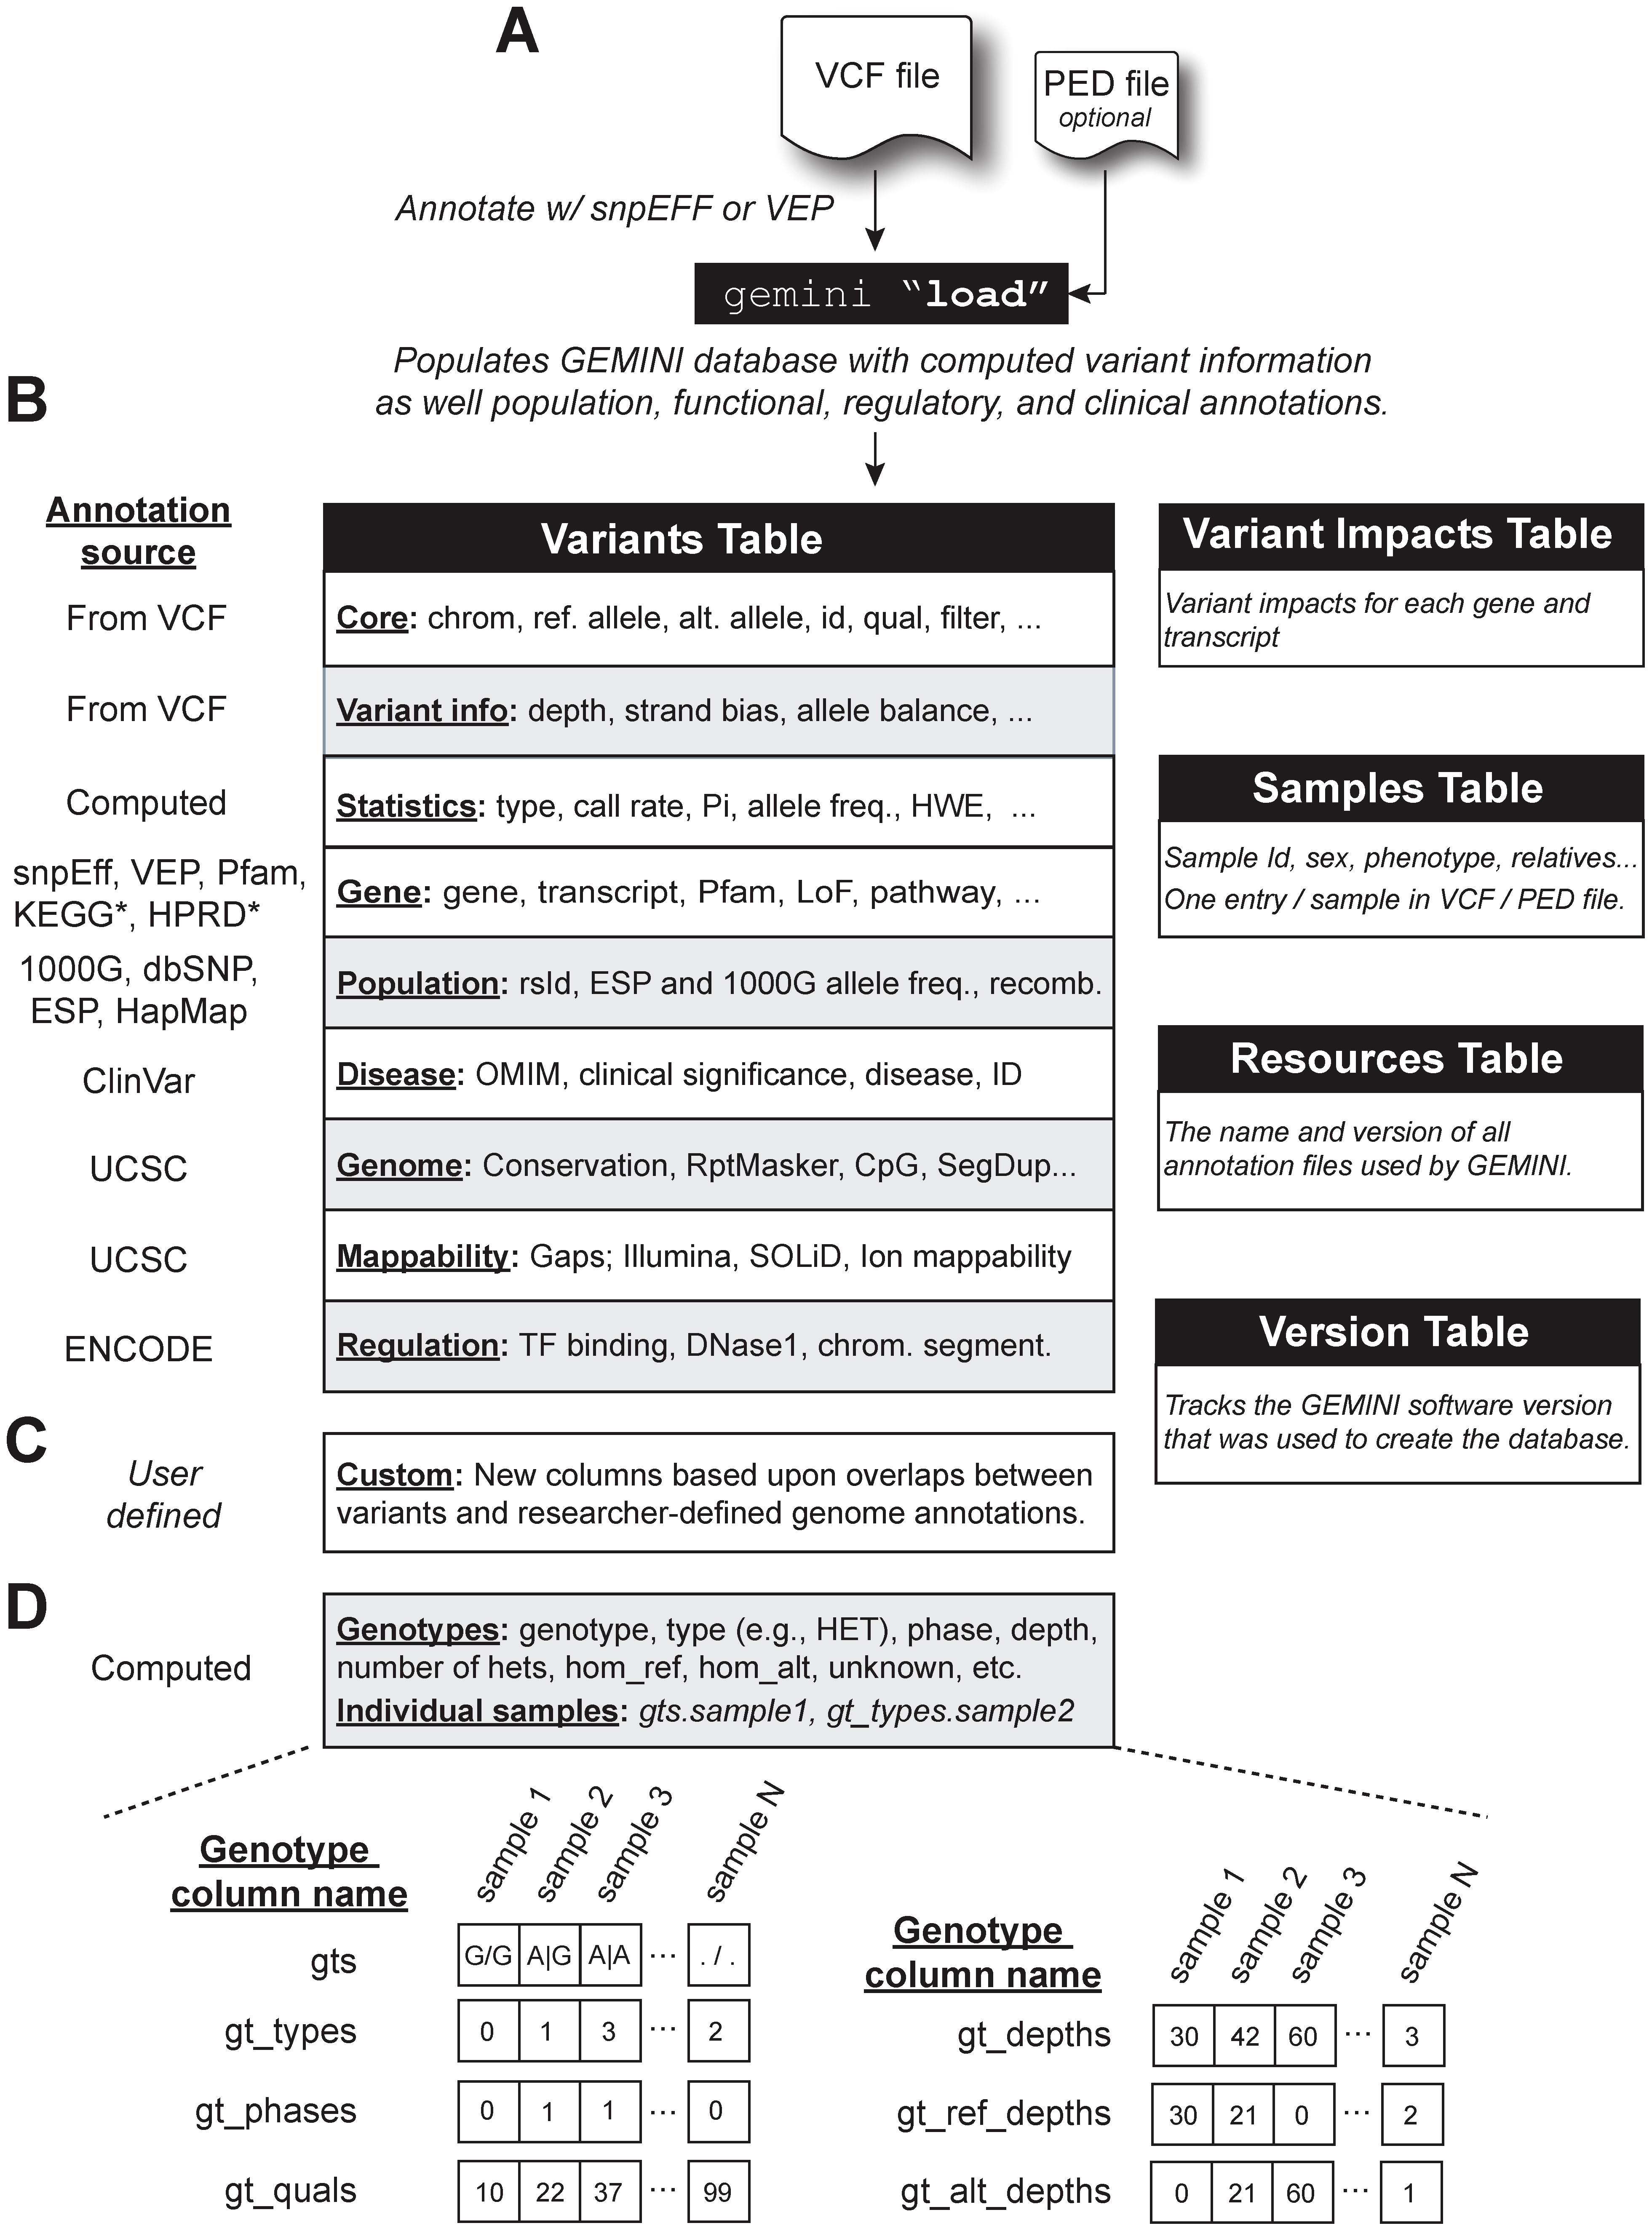
\includegraphics[width=\textwidth,height=\textheight,keepaspectratio]{gemini_schema}
\caption{Een overzicht van GEMINI's schema}
\label{gemini_schema_pic}
\end{figure}

\section{Inladen}
Het inladen van de data uit VCF-bestanden is een computationeel intensieve operatie, enerzijds omwille van de enorme grootte van deze bestanden, en anderzijds omdat in deze fase ook alle variants geannoteerd moeten worden. Om het proces te versnellen, biedt GEMINI de mogelijkheid het werk te paralleliseren door het VCF-bestand de comprimeren, op het bestaande bestand een index te defini\"eren en zo het werk te verdelen. Dit kan over meerdere processoren binnen 1 computer zijn, maar via de IPython-interface ook over volledige clusters van computers \cite{PER-GRA:2007}.\\

\section{Querying}

GEMINI laat de gebruiker toe de opgeslagen genoomdata te doorzoeken. Enerzijds via gewone SQL-queries, maar omdat het onderzoeken van individuele genotypes van cruciaal belang is in het onderzoek naar ziektes en SQL standaard niet de individuele genotypes in array-kolommen kan opvragen, biedt GEMINI bovendien een verrijkte SQL-syntax.\\
Zo laat het de gebruiker toe via filters en wildcards de gewenste genotype-eigenschappen en samples te specifi\"eren.

\subsection{Sample filters/wildcards} 
In SQL \texttt{SELECT}-statements kan de gebruiker met een filter van de vorm column.sample of een wilcard van de vorm (column).(wildcard) uitdrukken welke genotype-kolommen van welke samples hij/zij wilt zien. Wanneer de gebruiker ge\"interesseerd is in bijvoorbeeld het genotype van Jan, wordt dit:\\
\texttt{SELECT gt\_types.Bob FROM variants}\\\\
Als de gebruiker de diepte van de genotypes alle vrouwelijke samples wil zien, wordt dit:\\\\
\texttt{SELECT (gt\_depths).(sex = 'female')}.\\
GEMINI vertaalt de wildcard automatisch naar een query op de \texttt{samples}-tabel, en kan vervolgens voor alle samples die aan de voorwaarden voldoen, de waarde uit de gevraagde kolom tonen.

\subsection{Genotype filters/wildcards}
Om beperkingen op te leggen aan de variants waarin hij ge\"interesseerd is, kan de gebruiker SQL \texttt{WHERE}-clausules uitbreiden met zogenaamde genotype filters. Is de gebruiker bij voorbeeld enkel ge\"interesseerd in variants waarvoor Bob heterozygoot is en Bruce alles behalve heterozygoot is, kan dit met:\\

\noindent\texttt{\$ gemini query -q} "\texttt{SELECT * FROM variants}"\textbackslash \\\texttt{--gt-filter }"\texttt{gt\_types.Bob == HET and gt\_types.Bruce != HET}"\\

\noindent Vaak is het de bedoeling om eenzelfde beperking op te leggen aan meerdere samples. Op bovenstaande manier wordt dit al monikenwerk. Om dit te verhinderen, zijn er genotype wildcards van volgend formaat:\\ 
\texttt{(column).(sample\_wildcard).(gt\_wildcard\_rule).(rule\_enforcement)}.
\begin{description}
\item[column] Staat voor de genotype kolom waarop de beperking slaat.
\item[sample\_wildcard] Een wildcard om aan te duiden voor welke samples de beperking moet gelden. Analoog met de eerder vermelde sample wildcards.
\item[gt\_wildcard\_rule] De beperking op de genotype kolom.
\item[rule\_enforcement] Duidt aan hoeveel van de geselecteerde samples aan de opgelegde gt\_wildcard\_rule moeten voldoen. Dit kan \texttt{all, any, none, of count <comparison>} zijn.
\end{description}

\noindent Alle variants opvragen waarvoor alle mannen heterozygoot zijn, gaat bijvoorbeeld met:

\noindent\texttt{\$ gemini query -q "}\texttt{SELECT * FROM variants"}\textbackslash \\
\texttt{--gt-filter" }\texttt{(gt\_types).(sex = 'male').(=HET).(all)"}\\

\noindent Alle variants opvragen waarvoor minstens 1 bruinharig individu een genotype van diepte minstens 100 heeft, met:

\noindent\texttt{\$ gemini query -q "}\texttt{SELECT * FROM variants"}\textbackslash \\
\texttt{--gt-filter" }\texttt{(gt\_depths).(hair\_colour = 'brown').(>=100).(any)"}\\

\noindent Alle variants opvragen waarvoor minder dan 10 individu\"en een genotype met diepte minder dan 50 hebben, met:

\noindent\texttt{\$ gemini query -q "}\texttt{SELECT * FROM variants"}\textbackslash \\
\texttt{--gt-filter" }\texttt{(gt\_depths).(*).(=HET).(count < 10)"}\\

\noindent Al de bovenstaande filters kunnen met elkaar gecombineerd worden, evenals met gewone WHERE-clausules op de andere kolommen van de variants-tabel.

\subsection{\texttt{--show-samples}}

GEMINI biedt ook de mogelijkheid, bij een query op de \texttt{variants}-tabel, voor elke variant die aan de gestelde eisen voldoet, de namen van alle samples weer te geven die voor gegeven variant homozygoot of heterozygoot zijn. Dit gebeurt door de \texttt{--show-samples} flag mee te geven aan het \texttt{query} commando.




\chapter{Cassandra als databank voor GEMINI}
\label{concept}

Dit hoofdstuk belicht aan de hand van een case-study de conceptuele uitwerking van een schaalbare tool voor genoomanalyse. De case-study in kwestie is een versie van GEMINI die werkt met een Cassandra i.p.v. SQLite databank. Achtereenvolgens komen een motivatie voor de keuze voor Cassandra, de nodige aanpassingen aan het dataschema van GEMINI en de nodige aanpassingen aan GEMINI zelf om de inlaad- en querying-functionaliteit van GEMINI te behouden, aan bod.

\section{Keuze database}

\subsection{Vereisten}

Zoals beschreven in [\ref{gemini_beschrijving}] bewaart GEMINI de data over genetische varianten en proefpersonen in enkele zeer grote tabellen. Een eerste vereiste voor een database is dus om deze tabulaire data goed te kunnen voorstellen en beheren. Omdat de nadruk van dit onderzoek specifiek ligt op het schaalbaar maken van de applicatie, gebeurt dit bij voorkeur d.m.v. automatische verspreiding over verschillende nodes in een cluster.\\
Omdat GEMINI meerdere processoren of zelfs computers kan gebruiken bij het inladen van de gegevens uit VCF-bestanden, zijn goede concurrency-controle en hoge schrijfthroughput eveneens belangrijk. Na het inladen van de VCF bestanden voert GEMINI enkel nog leesqueries uit, dus zijn de belangrijkste verdere vereisten voor een database hoge leesthroughput, goede querymogelijkheden en indexeringsmechanismes die ook op een performante manier de verrijkte SQL-syntax van GEMINI ondersteunen.
\\Ten laatste is een Python-API ook nuttig, gezien GEMINI in Python ge\"implementeerd is.

\subsection{Keuze}

De uiteindelijke keuze voor een databank viel op Apache Cassandra. Van de systemen besproken in [\ref{nosql_survey}] heeft Cassandra veruit de meest interessante architectuur qua schaalbaarheid en bovendien verwachten we dat het columnaire model zich goed leent tot het modelleren van de tabellen in de oorspronkelijke versie van GEMINI, wat we dan ook experimenteel zullen valideren. Vergeleken met het andere columnaire systeem in de vergelijkende studie, HBase, heeft Cassandra uitgebreidere query-mogelijkheden. Vergeleken met MongoDB, dat sterker staat op het gebied van querying en indexing heeft Cassandra het voordeel dat het flexibeler is voor concurrent schrijven naar de databank. Bovendien blijkt uit eerdere experimenten met MongoDB binnen het lab dat MongoDB niet space-effici\"ent BSON-documenten kan uitbreiden.\\
In het geval van een incrementele versie van GEMINI, waar na verloop van tijd genoominformatie van extra proefpersonen ingeladen moet worden, leidt dit tot fragmentatie. Cassandra daarentegen kan eenvoudig het schema van tabellen aanpassen en naar behoefte extra kolommen en rijen toevoegen.

\section{Dataschema}

\label{cassandra_datamodel}

Het datamodel van Apache Cassandra vertoont enkele sterke verschillen met het relationele datamodel. Dit vereist enkele grondige aanpassingen aan het database schema van GEMINI. In deze sectie komen de belangrijkste eigenschappen van Cassandra aan bod, hun gevolgen voor de belangrijkste database-functionaliteiten, en een conceptuele schets van benodigde aanpassingen aan het onderliggende dataschema van GEMINI.

\subsection{Datamodel Cassandra}

Zoals eerder vermeld bewaart Cassandra de cellen in een tabel als een 2 dimensionele map van enerzijds een per rij gedefinieerde primary key, en de naam van een kolom. De inhoud van cellen die niet in de primary key van een rij liggen, heeft voor Cassandra geen enkele betekenis.\\
Die primary key bestaat uit 2 delen: het eerste is de partition key, deze bestaat uit minstens 1 kolom en de (gehashte) waarde hiervan bepaalt via het consistent-hashing mechanisme op welke partitie in de cluster de rij terechtkomt. Het tweede, optionele, deel is de clustering key, en bepaalt in welke volgorde rijen met dezelfde partition key op 1 node bewaard worden. Dit is standaard in oplopende volgorde.\\

Gezien Cassandra in essentie een grote map is, is de effici\"entste manier om rijen op te vragen uit een tabel eenvoudig de hash te berekenen van de primary key om vervolgens de passende rijen te returnen. De inhoud van kolommen buiten de primary key is ook volledig betekenisloos voor Cassandra en het individueel en iteratief inspecteren van cellen druist om performantieredenen in tegen de principes van Cassandra. Bij gevolg zijn de query-mogelijkheden eerder beperkt: zonder het defini\"eren van indices is het in \texttt{WHERE}-clausules enkel mogelijk beperkingen op te leggen aan kolommen in de primary key, en dan nog zo dat de bedoelde rijen binnen 1 partitie liggen, en opeenvolgend opgeslagen zijn. Daarom moet er een gelijkheidsbeperking opgelegd worden aan de volledige partition key, en mogen er zowel gelijk- als ongelijkheidsbeperkingen opgelegd worden aan de kolommen in de clustering key, maar enkel op voorwaarde dat de voorgaande kolom in de clustering key ook met een gelijkheidsbeperking gespecifieerd is. Op deze manier kan Cassandra queries zeer snel uitvoeren door ze a.d.h.v. de hash van de partition key naar een juiste node te routeren, en vervolgens via de overige opgegeven kolommen de locatie van de juiste rijen te berekenen (die omwille van de clustering allemaal op elkaar volgend opgeslagen zijn). Dit gebeurt zonder de waarden van individuele cellen te bekijken, maar dus enkel door het berekenen van een simpele hashfunctie. Range-queries zijn dus enkel mogelijk op kolommen in de clustering key en het is niet mogelijk \texttt{!=}-beperkingen te gebruiken in \texttt{WHERE}-clausules. Bovendien laat Cassandra enkel toe beperkingen met elkaar te combineren via conjuncties, dus niet via \texttt{OR}- of \texttt{NOT}-operatoren. Een uitzondering op dit laatste is de \texttt{IN}-operator: op deze manier kan de gebruiker meegeven in welke set van waarden een bepaalde kolom moet liggen, maar dit is ook enkel mogelijk op de laatste kolom in de partition key of de laatste kolom in de clustering key (maar weer op voorwaarde dat de voorgaande kolommen reeds beperkt zijn).\\
Cassandra laat toe om indices op kolommen te defini\"eren, maar die zijn niet bijzonder nuttig. Ze laten enkel gelijkheidsbeperkingen toe (dus geen range-queries) en bovendien raadt Datastax (die een enterprise-versie van Cassandra bouwen) het gebruik van indices op kolommen met zowel een zeer lage als een zeer hoge kardinaliteit af, dit omdat in het eerste geval de index tabel zal bestaan uit zeer weinig zeer lange rijen voor elk van de ge\"indexeerde waarden en in het tweede geval Cassandra bij een query op de ge\"indexeerde kolom door zeer veel verscheidene waarden zal moeten zoeken om een klein aantal resultaten te vinden \cite{when_to_use_index}.

\subsection{Databaseschema GEMINI}

Zoals blijkt uit bovenstaande beschrijving van het datamodel van Cassandra, leent het systeem zich niet goed tot ad-hoc querying: het is niet mogelijk op een performante manier zomaar aan willekeurige kolommen in een tabel voorwaarden op te leggen en deze voorwaarden met elkaar te combineren. Dit betekent dat bij het ontwerpen van het databaseschema al rekening gehouden moet worden met de queries die achteraf op de data mogelijk moeten zijn. Omdat het soort queries dat een tabel ondersteunt sterk samenhangt met de keuze van de primary key van de tabel en GEMINI meerdere, uiteenlopende soorten queries op elke tabel vereist, zal dit onvermijdelijk leiden tot duplicatie van data.\\
De belangrijkste queries die ondersteund moeten worden in GEMINI, zijn de volgende:
\begin{itemize}
\item Queries op de \texttt{variants}-tabel die genotype-eigenschappen van specifieke proefpersonen opvragen, al dan niet met behulp van sample-wildcards. Het moet ook mogelijk zijn voorwaarden op te leggen aan de genotypes van proefpersonen, met genotype-filters en -wildcards.
\item Normale SQL-achtige queries op arbitraire kolommen van de \texttt{variants}- en \texttt{samples}-tabellen.
\item Queries op \texttt{JOIN}s van tabellen. De documentatie van GEMINI heeft het in dit geval vooral over \texttt{JOIN}s tussen enerzijds de \texttt{gene\_detailed}- of \texttt{gene\_summary}-tabellen en anderzijds de \texttt{variants}- of \texttt{variant\_impacts}-tabellen \cite{gemini_joins}.
\end{itemize}
Deze drie vraagstukken komen achtereenvolgens aan bod in deze sectie.\\\\
In deze sectie komen meerdere schematische voorstellingen van databanktabellen voor. Om de leesbaarheid te verhogen, zijn hierin de namen van kolommen uit de partition key steeds in het {\color{ForestGreen} \underline{groen}} en van kolommen uit de clustering key in het {\color{red} rood} weergegeven.

\subsubsection{\texttt{variants}-tabel vs. genotype-informatie}

Het belangrijkste vraagstuk is hoe de genotype-kolommen uit het oorspronkelijke relationele model in Cassandra op te slaan. Hier zijn enkele opties voor:

\begin{itemize}

\item \textbf{Collection columns} Cassandra biedt zogenaamde collection types, zoals sets, lists of maps. Dit is vergelijkbaar met de bestaande implementatie in SQLite (buiten dat ze in Cassandra niet als binary blobs bewaard worden). Het nadeel is echter dat deze collections niet meer dan 65536 ($2^{16}$) entries kunnen bevatten, wat het hele nut van de migratie naar Cassandra, namelijk verhoogde schaalbaarheid, teniet zou doen.

\item \textbf{Super-\texttt{variants}-tabel} Een andere mogelijkheid is de \texttt{variants}-tabel uit te breiden met een kolom voor elke genotype-eigenschap van elke sample. Deze aanpak heeft als voornaamste voordeel dat de kolommen met genotype-eigenschappen van specifieke samples zonder omwegen uit de \texttt{variants}-tabel gehaald kunnen worden. Dit is vooral van belang voor de in (\ref{gemini_beschrijving}) beschreven sample-filters. Bovendien kan Cassandra tot 2 miljard cellen opslaan op 1 partitie, dus vormt het grote aantal kolommen dat dit model met zich meebrengt, geen probleem.\\

\begin{table}[!h]
\begin{adjustwidth}{-0.75in}{}
\begin{tabular}{@{}|l|l|l|l|l|l|l|l|l|l|@{}}
\toprule
\color{ForestGreen} \underline{variant\_id} & ref & alt & \ldots & gt\_types.alex & gt\_types.john & \ldots & gt\_depths.alex & gt\_depths.john & \ldots \\ \bottomrule
\end{tabular}
\end{adjustwidth}
\end{table}

Het nadeel is echter dat het onmogelijk is ad-hoc queries te defini\"eren op genotype-eigenschappen van willekeurige samples zonder het gebruik van secundaire indices. Elke query die in een \texttt{WHERE}-clausule andere kolommen of samples betrekt, vereist om de hierboven beschreven redenen een andere keuze van de primary key om effici\"ent de juiste rijen te kunnen opzoeken. Beschouw bijvoorbeeld deze twee queries:\\ 

\noindent\texttt{\$ gemini query -q} "\texttt{SELECT * FROM variants}"\textbackslash \\\texttt{--gt-filter }"\texttt{gt\_types.john == HET and gt\_depths.alex > 100}"\\

\noindent\texttt{\$ gemini query -q} "\texttt{SELECT * FROM variants}"\textbackslash \\\texttt{--gt-filter }"\texttt{gt\_types.john == HET and gt\_depths.tim > 75}"\\

De eerste vereist als primary key \texttt{((gt\_types.john),(gt\_depths.alex))}, terwijl de tweede \texttt{((gt\_types.john),(gt\_depths.tim))} vereist. Beide eisen zijn niet verzoenbaar, wat betekent dat hier twee verschillende tabellen met dezelfde data, maar andere primary keys nodig zijn.

\item \textbf{\texttt{genotype}-tabellen} Een derde optie is een \texttt{variants}-tabel zonder genotype-informatie, gecombineerd met een tabel voor elke eigenschap van de genotypes van de samples, met een rij voor elke \texttt{(variant, sample)}. Bijvoorbeeld:\\

\begin{itemize}

\item Een \texttt{variants\_by\_samples\_gt}-tabel met als primary key \texttt{((sample\_name, gt\_type), (variant\_id))}. De primary key is zo gekozen dat alle variants waarvoor een sample eenzelfde genotype heeft, bij elkaar op 1 node liggen, zodat deze gemakkelijk opgevraagd kunnen worden. Hetzelfde was mogelijk geweest met enkel \texttt{sample\_name} als partition key, maar met de bovenstaande, granulairdere partition key zijn de variants beter over de cluster verspreid. Bovendien houdt het vanuit een semantisch oogpunt geen steek range queries uit te voeren op de \texttt{gt\_type}-kolom, dus moet deze niet per se in de clustering key staan. De \texttt{variant\_id}-kolom ten slotte maakt enkel deel uit van de primary key om deze uniek te maken voor elk tupel \texttt{(variant, sample, genotype)}.\\

\begin{table}[!htbp]
\centering
\begin{tabular}{@{}|l|l|l|@{}}
\toprule
\color{ForestGreen} \underline{sample\_name} & \color{ForestGreen} \underline{genotype} & \color{red} variant\_id \\ \bottomrule
\end{tabular}\\
\end{table}

\item Een \texttt{variants\_by\_samples\_gt\_depth}-tabel met als primary key \texttt{((sample\_name), (gt\_depth, variant\_id))}. Omdat range queries op de \texttt{gt\_depth}-kolom wel een vereiste zijn, moeten alle variants voor eenzelfde sample volgens gt\_depth geclusterd, en dus gerangschikt staan. Vandaar dat de \texttt{gt\_depth}-kolom in dit geval in de clustering key, en niet in de partition key staat. Voor de rest is de keuze van de primary key volledig analoog met die in de \texttt{variants\_by\_samples\_gt}-tabel.

\begin{table}[!htbp]
\centering
\begin{tabular}{@{}|l|l|l|@{}}
\toprule
\color{ForestGreen} \underline{sample\_name} & \color{red} gt\_depth & \color{red} variant\_id \\ \bottomrule
\end{tabular}
\end{table}

\item Vergelijkbare tabellen voor de overige genotype-eigenschappen.

\end{itemize}

Het grote voordeel van deze aanpak is dat het, dankzij de keuze van de primary key, zeer eenvoudig is variants op te vragen waarvoor het genotype van \'e\'en sample aan specifieke gelijkheids- of ongelijkheidsvoorwaarden voldoet. Het nadeel van dit schema is drieledig: ten eerste scheidt het de informatie over de genotypes van samples van de andere informatie over de variants. Dit betekent dat, om deze samen weer te geven, een \texttt{JOIN} van de \texttt{variants}-tabel met een \texttt{genotype}-tabel nodig is, en Cassandra biedt zoals geweten geen \texttt{JOIN}s. Ten tweede is het onmogelijk om met een sample-filter voor meerdere samples de genotypes tegelijkertijd op te vragen, en ten laatste is het onmogelijk in een query voorwaarden op te leggen aan de genotypes van meerdere samples.

\item \textbf{Super-\texttt{variants}-tabel + \texttt{genotype}-tabellen}
Een vierde mogelijke strategie is de combinatie van de tweede en de derde optie. Dit leidt tot nog meer dataduplicatie, maar bewaart wel de mogelijkheid om zowel genotype-informatie van willekeurige samples op te vragen door middel van de sample-filters als de \texttt{variants}-tabel te doorzoeken met, dankzij gt-filters en -wildcards, beperkingen op de genotypes van specifiek gekozen samples.

\end{itemize}

De uiteindelijke keuze is gevallen op de laatste optie, omdat die het meest van de 4 de queryfunctionaliteiten van GEMINI ondersteunt. Zoals hierboven beschreven blijft het zelfs met dit dataschema niet voor de hand liggend alle in GEMINI mogelijke queries uit te voeren, en zal door het ontbreken van \texttt{JOIN}s en de layout van de \texttt{genotype}-tabellen het combineren van beperkingen op de genotypes van meerdere samples nog extra aanpassingen vergen. Hier gaan secties \ref{gemini_query_concept} en \ref{gemini_query_impl} uitvoerig op in.

\subsubsection{\texttt{variants-, samples-}tabel vs. arbitraire queries}
\label{arbitraire_queries}

Een tweede belangrijk vraagstuk is hoe de \texttt{variants-} en \texttt{samples-}tabellen zo te ontwerpen dat ze ook op andere, arbitraire kolommen effici\"ent doorzoekbaar zijn.\\
Om queries op kolommen te ondersteunen die logisch gezien enkel met gelijkheden beperkt zullen worden, zoals \texttt{chrom} of respectievelijk \texttt{sex}, zou het in theorie volstaan op deze kolommen een secundaire index te defini\"eren. Dit is eenvoudig bij de creatie van de tabel, veroorzaakt geen duplicatie van data en is zeer rechttoe rechtaan bij het queryen, maar heeft zoals hierboven vermeld onvoorspelbare performantie afhankelijk van de kardinaliteit van de kolommen. Bovendien werkt dit mechanisme niet voor kolommen die vaker met ongelijkheidsbeperkingen gequeried zullen worden, zoals \texttt{depth}, \texttt{start}, of in het geval van de \texttt{samples}-tabel (hypothetisch, deze tabellen zitten niet standaard in GEMINI) leeftijd of generatie.\\

Een aanpak die in beide gevallen op een voorspelbare en betrouwbare manier werkt, is om net als voor de genotype-informatie extra hulptabellen te defini\"eren, met een specifiek gekozen primary key die de gewenste query mogelijk maakt. Deze oplossing zorgt natuurlijk voor veel gedupliceerde data, maar heeft als voordeel dat ze \'e\'en coherente en performante aanpak van het probleem mogelijk maakt. Bij het opstellen van deze hulptabellen moet goed overwogen worden welke vaakgebruikte queries een eigen hulptabel vereisen en verdienen. Minder frequente, uitgebreidere queries, kunnen mits een goede keuze van de basishulptabellen immers gesplitst worden in subqueries op deze basishulptabellen. Hetzelfde mechanisme dat voor de gt-filters en -wildcards uitgebreide queries zal uitvoeren is ook hier van toepassing. Dit zal natuurlijk minder effici\"ent zijn dan een aangepaste hulptabel voor de uitgebreide, originele query, maar laat toe de gegevensduplicatie enigszins binnen de perken te houden. Voorbeelden van zulke basishulptabellen zijn:

\begin{itemize}
\item Een \texttt{variants\_by\_chrom\_start}-tabel, die het eenvoudig maakt alle varianten op te zoeken die op een bepaald chromosoom binnen een range van startposities liggen. De primary key is in dit geval: \texttt{((chrom), (start, variant\_id))}. 

\begin{table}[!htbp]
\begin{tabular}{@{}|l|l|l|@{}}
\toprule
\color{ForestGreen} \underline{chrom} & \color{red} start & \color{red} variant\_id \\ \bottomrule
\end{tabular}
\end{table}

\item Een \texttt{variants\_by\_gene}-tabel, die het eenvoudig maakt alle varianten binnen \'e\'en gen op te zoeken. De primary key is in dit geval: \texttt{((gene), (variant\_id))}.

\begin{table}[!htbp]
\begin{tabular}{@{}|l|l|@{}}
\toprule
\color{ForestGreen} \underline{gene} & \color{red} variant\_id \\ \bottomrule
\end{tabular}
\end{table}

\item Een \texttt{samples\_by\_sex}-tabel, die het eenvoudig maakt alle samples van een bepaald geslacht op te vragen. De primary key is in dit geval: \texttt{((sex), (sample\_name))}.

\begin{table}[!htbp]
\begin{tabular}{@{}|l|l|@{}}
\toprule
\color{ForestGreen} \underline{sex} & \color{red} sample\_name \\ \bottomrule
\end{tabular}
\end{table}
\end{itemize}

De enige soort queries die onze implementatie niet ondersteunt, zijn pure range-queries, zoals:\\

\texttt{SELECT * FROM variants WHERE start > 123456}\\\\
Zoals eerder beschreven in \ref{cassandra_datamodel} laat het datamodel van Cassandra dit niet toe: het is op basis van de query onmogelijk een primary key te bepalen van de rijen in het resultaat om zo een set opeenvolgende rijen uit de tabel in kwestie op te vragen. Een mogelijke oplossing is om een hulptabel te defini\"eren met als partition key een kolom met beperkte kardinaliteit, zoals \texttt{chrom} (de mens heeft slechts 46 chromosomen, zie \ref{dna_dummies}) en als clustering column de kolom waarop range queries nodig zijn, in dit geval \texttt{start}. In de client code kan bovenstaande range query dan vertaald worden naar 46 range queries die voor elk chromosoom de variant binnen de bepaalde range opvragen.   

\subsubsection{\texttt{JOIN}s}

Zoals eerder aangehaald, biedt Cassandra geen \texttt{JOIN}s in de bijhorende querytaal CQL. In de plaats moedigt Cassandra het \textit{materializen} van \texttt{JOIN}s aan, namelijk het samen bewaren van gegevens die samen opgevraagd zullen worden. Dit leidt tot de denormalizatie t.o.v. relationele dataschema's, die ontworpen zijn om zo opslageffici\"ent mogelijk alle data voor te stellen en zwaar inzetten op \texttt{JOIN}s om gegevens uit verschillende tabellen met elkaar te combineren.\\
GEMINI biedt de gebruiker ook de optie verschillende tabellen samen te doorzoeken m.b.v. \texttt{JOIN}s. Enkele voorbeelden zijn:

\lstinputlisting[language=SQL]{vb_SQL_queries/joins.txt}

Dankzij het hierboven beschreven query-mechanisme is het echter niet nodig alle tabellen die met elkaar gejoind zouden kunnen worden, ook effectief samen op te slaan in 1 tabel. Door alweer juist gekozen hulptabellen te defini\"eren, kunnen het reeds uitgelegde datamodel en query-mechanisme ook hier van dienst zijn.\\
Om de eerste van de twee queries uit bovenstaand voorbeeld uit te voeren, is dan bijvoorbeeld een tabel nodig die het mogelijk maakt alle variants met een bepaalde \texttt{impact\_severity} op te vragen (bvb. \texttt{variants\_by\_impact\_severity}), en een tweede tabel die toelaat alle genen uit \texttt{gene\_detailed} op te vragen voor een bepaalde waarde van de \texttt{gene} en \texttt{chrom} kolommen (bvb. \texttt{gene\_detailed\_by\_gene\_chrom}). De gewenste variants kunnen opgehaald worden uit de \texttt{variants\_by\_impact\_severity}-tabel en vervolgens kunnen via de \texttt{gene\_detailed\_by\_gene\_chrom} alle gewenste kolommen uit de \texttt{variants}- en \texttt{gene\_detailed}-tabellen geselecteerd worden. Een analoge redenering gaat op voor de tweede voorbeeldquery en bij uitbreiding ook voor de andere voor GEMINI relevante \texttt{JOIN}s \cite{gemini_joins}.

\section{\texttt{gemini load}}

Het inladen van de genoomdata in de GEMINI-databank is conceptueel erg eenvoudig: elke lijn uit een VCF-file komt overeen met een variant en dus een rij in de \texttt{variants}-tabel (en de bijhorende hulptabellen), elke lijn in een PED-file met een sample en dus een rij in de \texttt{samples}-tabel (en de bijhorende hulptabellen). Het inladen kan bovendien versneld worden door de text-input te verdelen over verschillende cores en deze in parallel de data te laten invoeren.

\section{\texttt{gemini query}}
\label{gemini_query_concept}
Het uitvoeren van de gewoonlijke GEMINI-queries tegen een Cassandra-databank vergt enkele ingrijpende aanpassingen ten opzichte van de SQLite-versie van Cassandra. Het doel is natuurlijk deze aanpassingen zoveel mogelijk te verbergen voor de gebruiker, wat ook in grote mate gelukt is. In deze sectie komt achtereenvolgens aan bod hoe ingewikkelde queries gesplitst worden in eenvoudige subqueries, hoe de resultaten hiervan vervolgens gecombineerd worden en wat dit betekent voor de meest geavanceerde feature van GEMINI, namelijk de genotype-filters en -wildcards.

\subsection{Splitsing in subqueries}
\label{splitsing_subqueries_conceptueel}

Zoals beschreven in \ref{cassandra_datamodel}, kan Cassandra enkel effici\"ent queries uitvoeren die beperkingen opleggen aan de kolommen in de primary key van een tabel, en dit ook slechts onder bepaalde voorwaarden. Bovendien is de enige logische operator die Cassandra ondersteunt om beperkingen te combineren, de conjunctie.\\
Om arbitraire queries en \texttt{WHERE}-clausules te ondersteunen, kan GEMINI niet zoals in de SQLite-versie de \texttt{WHERE}-clausule zomaar onveranderd aan Cassandra doorgeven. Beschouw, ter illustratie, volgende query:\\\\
\texttt{SELECT chrom, start, subtype FROM variants WHERE chrom = 'chromX' \\AND start > 5600 AND gene = 'gene\_A'}.\\\\
Deze query valt uiteen in 2 subqueries: een eerste om uit de \texttt{variants\_by\_chrom\_start}-tabel alle variants op te vragen die voldoen aan de voorwaarde \texttt{chrom = 'chromX' AND start > 5600} en een tweede om uit de \texttt{variants\_by\_gene}-tabel alle variants die voldoen aan \texttt{gene = 'gene\_A'} op te vragen. Deze subqueries zullen uit de hulptabellen enkel de primary keys opvragen van de rijen die aan de voorwaarden voldoen, in dit geval de \texttt{variant\_id} van de variants. De overige opgevraagde kolommen, \texttt{chrom, start, subtype} moeten achteraf met deze primary keys opgehaald worden uit de \texttt{variants}-hoofdtabel.\\

\subsection{Combineren subqueries}
\label{comb_subq_concept}
De subqueries zullen elk een verzameling primary keys van rijen als resultaat opleveren. Het is dan zaak deze verzamelingen met set-operaties te combineren tot de finale verzameling primary keys van rijen die aan de query voldoen. De nodige set-operatie hangt af van de oorspronkelijke query. Zo zal het eindresultaat van een conjunctie van subqueries de doorsnede van de resultaatverzamelingen van de subqueries zijn. In het geval van een disjunctie is dit de unie van de resultaatverzamelingen, en in het geval van een negatie van een subquery is dit het verschil tussen de oorspronkelijke verzameling (voor de query) en de resultaatverzameling van de query. Om bijvoorbeeld alle varianten te vinden die niet op een bepaald gen x liggen, moet het verschil bepaald worden tussen de verzameling van alle varianten en de verzameling van alle varianten die op gen x liggen. Tabel \ref{combineren_subqueries} vat dit samen voor 2 subqueries $p$ en $r$, hun respectievelijke resultaatverzamelingen $res(p)$ en $res(r)$ en een initi\"ele verzameling rijen $I$.

\begin{table}[h]
\centering
\begin{tabular}{|l|l|}
\hline
\textbf{Query} & \textbf{Resultaat}    \\ \hline
$p$ \texttt{AND} $r$ & $res(p) \cap res(r)$   \\ \hline
$p$ \texttt{OR} $r$ & $res(p) \cup res(r)$    \\ \hline
\texttt{NOT} $p$  & $I \setminus res(p)$ \\ \hline
\end{tabular}
\caption{De verschillende manieren om subqueries met elkaar te combineren.}
\label{combineren_subqueries}
\end{table}

\subsection{Ophalen finaal resultaat}

Met het resultaat van de subqueries, namelijk de primary keys van alle rijen uit de oorspronkelijk gevraagde (hoofd)tabel die voldoen aan de query, is het eenvoudig het eindresultaat van de query te bepalen. Er is nog \'e\'en query nodig die voor alle rijen de gevraagde kolommen opvraagt uit de hoofdtabel. Ook hier is er een mogelijkheid om door parallellisatie het proces te versnellen: de verzameling primary keys kan over meerdere processoren verdeeld worden, die dan elk een deel van het eindresultaat voor hun rekening nemen. 

\subsection{Genotype-filter wildcards}

Ter herinnering, de structuur van een genotype-filter wildcard:\\\\
\texttt{(genotype\_column).(sample\_wildcard).(gt\_wildcard\_rule).(rule\_enforcement)}\\\\
Het uitvoeren en evalueren van deze wildcards is conceptueel niet erg ingewikkeld: het volstaat de \texttt{sample\_wildcard} te evalueren en vervolgens voor elk van de resulterende samples een subquery op te stellen op de voor \texttt{genotype\_column} relevante hulptabel van de \texttt{variants}-tabel. Hoe deze subqueries met elkaar gecombineerd moeten worden, hangt af van de gegeven \texttt{rule\_enforcement}:

\begin{itemize}
\item Een \texttt{all}-wildcard leidt tot de conjunctie van alle subqueries.
\item Een \texttt{any}-wildcard leidt tot de disjunctie van alle subqueries.
\item Een \texttt{none}-wildcard leidt tot de conjunctie van de negaties van alle subqueries.
\item \texttt{count}-wildcards vallen niet zomaar met set-algebra te evalueren: bij het combineren van de resultaten van alle subqueries moet voor elke variant geteld worden in de resultaatverzameling van hoeveel subqueries hij voorkomt. Nadien kan GEMINI eenvoudig op basis van deze tellingen de varianten bepalen die aan de \texttt{count}-regel voldoen.
\end{itemize}

Dit betekent dat weer veel werk van de databank naar GEMINI zelf verschuift. Een mogelijke manier om dit leed te verzachten is, gezien de goede concurrency-eigenschappen van NoSQL-systemen als Cassandra, om de subqueries in parallel te evalueren in plaats van sequentieel.

\section{Conceptueel ontwerp: conclusie}

Bij wijze van gevalstudie voor schaalbare genoomanalyse hebben we een versie van GEMINI draaiende op Apache Cassandra ontworpen. Cassandra droeg onze voorkeur uit omwille van een uitstekende reputatie qua schaalbaarheid, een flexibel datamodel dat goed bij GEMINI past en een gemakkelijk te gebruiken querying API. Voor de omzetting van SQLite naar Cassandra waren enkele aanpassingen aan het ontwerp van GEMINI nodig: vooral aan het databaseschema en het queryingmechanisme, in mindere mate aan de loading-functionaliteit. Hoofdstuk \ref{implementatie} bespreekt de praktische implementatie van dit ontwerp.

\chapter{Cassandra \& GEMINI: implementatie}
\label{implementatie}

Dit hoofdstuk beschrijft de praktische realisatie van een versie van GEMINI draaiende op Cassandra in de plaats van SQLite, verderbouwend op het ontwerp uit hoofdstuk \ref{concept}. De implementatie is gebaseerd op versie 0.1.11 van GEMINI, 2.1.4 van Apache Cassandra en versie 2.5.1 van de Python driver voor Cassandra, ontwikkeld door DataStax \cite{cassandra_driver}. 

\section{\texttt{gemini load} met Cassandra}
Het inladen van genoomdata in GEMINI gebeurt in twee stappen. De reden voor die opsplitsing is dat een klein deel van het inladen en initialiseren van de databank niet parallel op meerdere processoren kan verlopen. \\In de eerste en kleinste van de twee, initialiseert GEMINI de databank, maakt de nodige tabellen aan en laadt de samples-informatie in. GEMINI haalt de namen van de samples uit de VCF-file, en vult die aan met informatie uit de PED-file. Indien er geen PED-file voorhanden is, initialiseert GEMINI de \texttt{samples}-tabel met default-waarden voor de kolommen zoals \texttt{sex} en \texttt{phenotype}. Meteen worden ook de extra, aan de \texttt{samples}-tabel verbonden tabellen zoals \texttt{samples\_by\_sex} en \texttt{samples\_by\_phenotype} aangemaakt en gevuld. Ook de \texttt{resources-, gene\_detailed-, gene\_summary-} en \texttt{version-}tabellen worden in de eerste fase gevuld. Dit omdat de pedigree-files en de bestanden met data over de genen niet effici\"ent opgesplitst kunnen worden. Bovendien is de duur van het inladen van de \texttt{samples}-tabel zelfs bij 10000'en samples verwaarloosbaar tegenover het inladen en annoteren van de \texttt{variants}-tabel.\\
In de tweede fase gebeurt het leeuwendeel van het werk: het inladen van de variants-informatie uit de (verplicht meegegeven) VCF-file. Dankzij de bgzip \cite{bgzip} en grabix \cite{grabix} tools kan GEMINI effici\"ent VCF-bestanden in blokken opsplitsen, comprimeren, hierop een index defini\"eren en vervolgens daarmee verderwerken. Zo kan GEMINI eenvoudig het inladen van de variants, die elk \'e\'en lijn in de VCF-file in beslag nemen, gemakkelijk over meerdere cores verdelen. Het is ook in deze fase dat GEMINI de aan de \texttt{variants}-tabel verwante tabellen zoals \texttt{variants\_by\_samples\_gt\_type}, \texttt{variants\_by\_samples\_gt\_depth} en \texttt{variants\_by\_chrom\_start} opvult. Alle cores of nodes in het cluster, voeren rechtstreeks rijen in in \'e\'en en dezelfde tabel in de Cassandra-databank. Omdat Cassandra atomiciteit binnen rijen garandeert en alle workers strikt disjuncte sets van variants invoeren in het systeem, is er geen enkel risico op conflicten.\\\\
De grote winst ten opzichte van de SQLite-implementatie van GEMINI is dat in het parallelle gedeelte, alle workers naar dezelfde databank kunnen schrijven. In de SQLite-versie van GEMINI schrijven alle workers naar een aparte SQLite-database, die vervolgens in een kostelijke operatie nog allemaal samengevoegd moeten worden tot \'e\'en grote SQLite-databank. Die stap (het \texttt{gemini merge}-commando) kan de Cassandra-implementatie volledig overslaan. Een ander opzicht waarin de Cassandra-implementatie effici\"enter is dan de SQLite-versie, is dat in SQLite voor elke variant de genotype-kolommen nog tot binary blobs gecomprimeerd worden. In Cassandra is dit, dankzij de keuze van het databaseschema, niet nodig.

\section{\texttt{gemini query} met Cassandra}
\label{gemini_query_impl}

\subsection{Splitsing in subqueries}


Om zoals in het voorbeeld uit \ref{splitsing_subqueries_conceptueel} dynamisch beslissingen over het splitsen in subqueries te kunnen maken, is het nodig de \texttt{WHERE}-clausule te inspecteren en hieruit de benodigde hulptabellen voor de subqueries te identificeren. Om dit proces te vereenvoudigen, hanteert deze implementatie een licht gewijzigde querysyntax: beperkingen die binnen 1 hulptabel liggen, kunnen nog steeds met elkaar gecombineerd worden met het \texttt{AND}-keyword, maar beperkingen die niet binnen eenzelfde hulptabel liggen, moeten met de \texttt{\&\&, ||} of \texttt{NOT}-operatoren van elkaar gescheiden worden. Zo kan GEMINI bij het parsen van de \texttt{WHERE}-clausule deze onmiddellijk opsplitsen in subqueries en voor elk van deze subqueries de nodige hulptabel bepalen. Beschouw wederom volgende query:\\\\
\texttt{SELECT chrom, start, subtype FROM variants WHERE chrom = 'chromX' \\AND start > 5600 AND gene = 'gene\_A'}.\\\\
In de aangepaste syntax wordt dit:\\\\
\texttt{SELECT chrom, start, subtype FROM variants WHERE chrom = 'chromX' \\AND start > 5600 \&\& gene = 'gene\_A'}.\\

Dit vereist uiteraard dat de gebruiker op de hoogte is van welke hulptabellen er bestaan. Gebruikers moeten sowieso weten op welke kolommen ze queries kunnen defini\"eren, en bijgevolg ook welke hulptabellen er bestaan. Bovendien bestaat het doelpubliek van GEMINI uit onderzoekers die het programma intensief gebruiken en dus voldoende gelegenheden hebben om dergelijke aanpassingen snel onder de knie te krijgen.\\
%TODO
Een andere optie is de syntax onveranderd te laten en uit de in de \texttt{WHERE}-clausule vermelde kolommen benodigde hulptabellen af te leiden. Die aanpak heeft als voordeel dat de interface naar de gebruiker niet verandert, maar gezien nog steeds enkel queries mogelijk zijn op kolommen uit de hoofdtabel waarvoor hulptabellen bestaan, is achterwaartse compatibiliteit hiermee nog niet verzekerd. Daarbovenop levert ze ook nieuwe problemen op, zoals: wat met kolommen die in meerdere hulptabellen voorkomen, welke combinatie van tabellen wordt er dan best geselecteerd? Dergelijke vraagstukken neigen naar query-optimization en vallen buiten het ... {\color{red} TODO} Daarom verkoos ik de macht bij de gebruiker te leggen en te vertrouwen op diens oordeelkundigheid.\\\\
De gebruiker dient er ook rekening mee te houden dat Cassandra range-queries enkel onder strikte voorwaarden ondersteunt, namelijk (zoals eerder uitgelegd) enkel op clustering columns en enkel wanneer de voorgaande kolommen in de clustering key met gelijkheden beperkt zijn. Dit impliceert dat er slechts een range query op 1 kolom in een tabel mogelijk is. Daarnaast biedt Cassandra ook geen \texttt{!=}-operator. Dit euvel valt te verhelpen door een \texttt{!=}-clausule om te zetten naar een gelijkheidsbeperking en die vervolgens te negeren. Een clausule als \texttt{phenotype != 2} wordt dan \texttt{NOT (phenotype = 2)}. Dit vereist dat de \texttt{!=}-clausule een aparte subquery vormt.\\

Het uiteindelijke algoritme om de geschikte hulptabel te selecteren op basis van de kolommen en gebruikte operatoren in een subquery, gebruikt de metadata van het Cassandra-cluster om alle hulptabellen voor een gegeven hoofdtabel op te vragen, en vervolgens aan de hand van de kolommen in de primary keys van de kandidaat-hulptabellen de geschikte eruit te kiezen.\\

GEMINI encapsuleert de subqueries in \texttt{query\_expression}s: een set Python-klassen die, ge\"inspireerd door algebra\"ische datatypes uit functionele talen zoals Haskell, alle mogelijke GEMINI-queries kunnen voorstellen. Die bevatten alle informatie die GEMINI nodig heeft om de queries te evalueren. De \texttt{Basic\_expression} stelt een eenvoudige query op een Cassandra-tabel voor. Tijdens het parsen van de \texttt{WHERE}-clausule zal GEMINI de subqueries inkapselen in \texttt{Basic\_expressions} en die, afhankelijk van de gehele query, nesten in \texttt{AND\_}-, \texttt{OR\_}- of/en \texttt{NOT\_expression}s. De \texttt{GT\_wildcard\_expression} stelt op een effici\"ente manier genotype-filter wildcards voor (zie \ref{gt_wildcards}). De volgende paragraaf bespreekt in detail de aangeboden \texttt{evaluate}- en \texttt{can\_prune}-functies.

\begin{figure}[h]
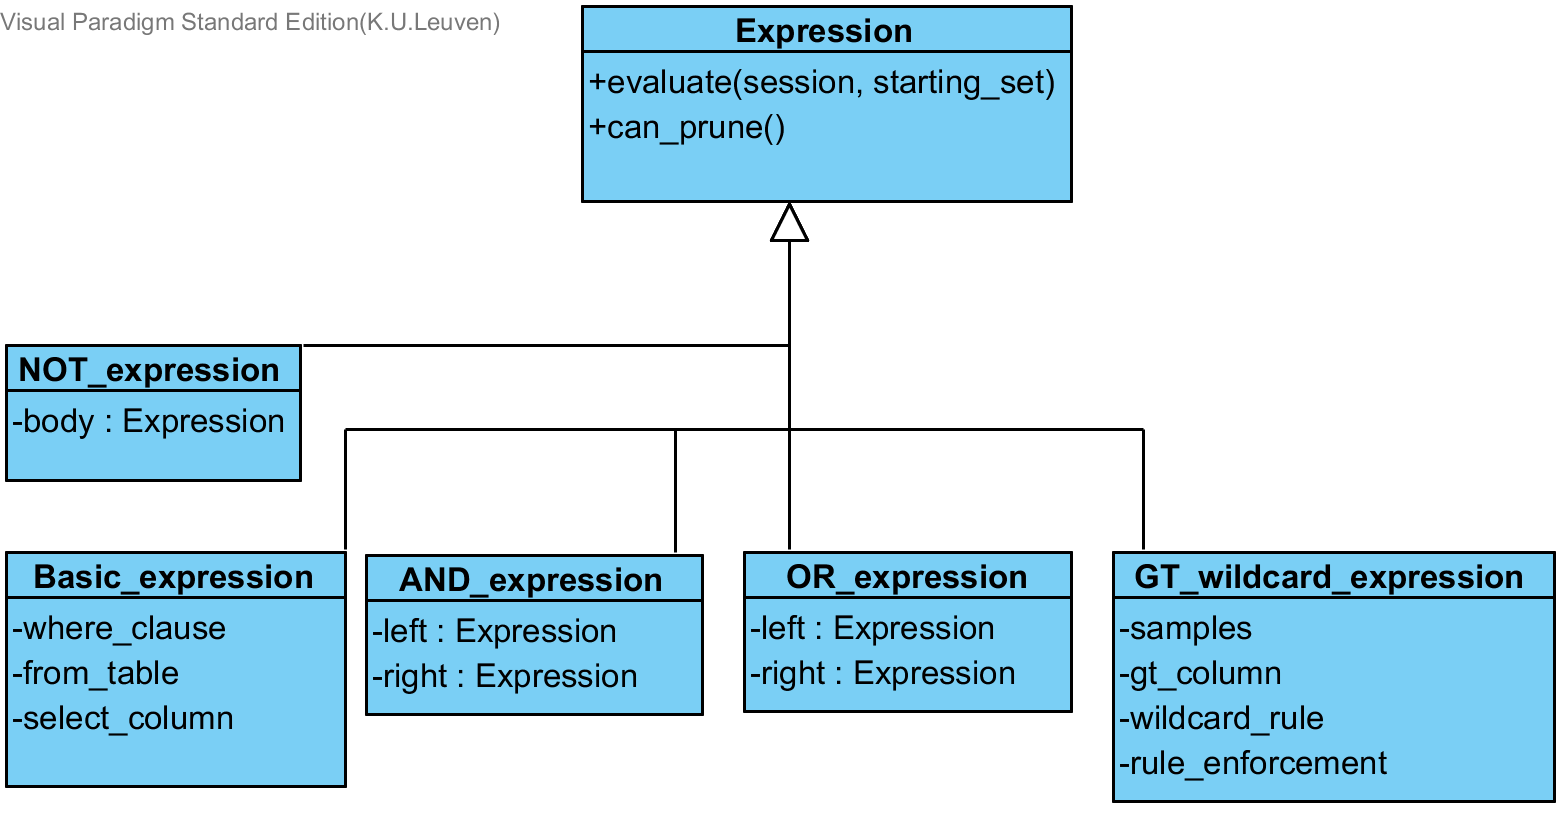
\includegraphics[width=\textwidth,height=\textheight,keepaspectratio]{query_exps}
\caption{De \texttt{query\_expressions} waarmee alle queries gemodelleerd worden. Het \texttt{session}-argument van de \texttt{evaluate}-functie is een actieve verbinding met het Cassandra-cluster.}
\label{query_exps_diagram}
\end{figure}

\subsection{Combineren subqueries}

Uit performantie-overwegingen is het een logische keuze de resultaten van subqueries op de hulptabellen te bewaren in een set datatype. Zo kunnen de benodigde set-operaties gebruik maken van de in Python ingebouwde set-operaties en zo veel effici\"enter verlopen dan wanneer de resultaten in bijvoorbeeld lists bewaard worden. Het enige nadeel van sets t.o.v. lists is dat de implementatie geen garanties biedt over in welke volgorde rijen in het eindresultaat zullen voorkomen. Dit weegt niet op tegen de tijdswinst, en bovendien biedt Cassandra zelf (in de algemeen aangeraden consistent hashing-partitionering) geen enkele garantie over in welke volgorde het rijen opslaat.\\\\
Bij het praktisch evalueren van \texttt{query\_expression}s komt uiteindelijk meer kijken dan enkel set-operaties. De belangrijkste reden hiervoor is dat, zoals in \ref{comb_subq_concept} reeds beschreven, om een negatie of \texttt{NOT\_expression} te kunnen evalueren, alle kandidaat-rijen gekend moet zijn, en dus meegegeven aan de \texttt{evaluate}-functie. Die extra informatie kan ook bij het evalueren van andere types van \texttt{query\_expression} goed van pas komen.
 
\begin{itemize}
\item Het evalueren van \texttt{Basic\_expression}s gebeurt niet zo rechtoe rechtaan als de naam doet vermoeden. De \texttt{evaluate}-functie bouwt een CQL-query op, op basis van een gegeven \texttt{WHERE}-clausule, de relevante tabel en de gevraagde kolom uit die tabel. Wanneer er een zinvolle verzameling kandidaatrijen (de \texttt{starting\_set} in onderstaand codefragment) meegegeven is, wordt die als \texttt{IN}-clausule aan de \texttt{WHERE}-clausule toegevoegd. Zo zoekt Cassandra enkel in rijen die effectief in aanmerking komen om aan de globale query te voldoen. Een voorwaarde om die optimalisatie te kunnen toepassen, is dat de \texttt{WHERE}-clausule geen ongelijkheidsbeperkingen mag bevatten (vandaar de \texttt{can\_prune}-functie).

\lstinputlisting[language=Python,firstline=31,lastline=48]{gemini_src/query_expressions.py}

\item Om een \texttt{AND\_expression} te evalueren is het strikt genomen nodig beide leden van de uitdrukking te evalueren en vervolgens de doorsnede te nemen van de resultaten. Als \'e\'en van de twee leden van de uitdrukking echter in staat is om dankzij een CQL \texttt{IN}-clausule enkel naar rijen te zoeken die effectief in aanmerking komen om aan de globale query te voldoen, is het mogelijk om die operatie aan Cassandra over te laten. Als het rechterlid kan \textit{prunen}, dan kan GEMINI de resultaatverzameling van het linkerlid als \texttt{starting\_set} meegeven bij de evaluatie van het rechterlid, en omgekeerd. Wanneer geen van beide kunnen \textit{prunen}, moet GEMINI uiteraard nog steeds zelf de doorsnede berekenen.

\lstinputlisting[language=Python,firstline=56,lastline=66]{gemini_src/query_expressions.py}

\item In het geval van een \texttt{OR\_expression} is er geen andere mogelijkheid dan eenvoudigweg het linker- en rechterlid te evalueren, beide met als \texttt{starting\_set} de \texttt{starting\_set} van de \texttt{OR\_expression} zelf, en vervolgens de unie van de resultaten te berekenen.

\item Ook in het geval van een \texttt{NOT\_expression} is er geen andere optie dan de \texttt{body}-uitdrukking te evalueren en vervolgens het complement van de \texttt{starting\_set} en het resultaat te bepalen. Als de gegeven \texttt{starting\_set} gelijk is aan \texttt{"*"}, d.w.z. alle rijen in de oorspronkelijke tabel, zit er ook niets anders op dan die nog eerst allemaal op te vragen.

\lstinputlisting[language=Python,firstline=101,lastline=110]{gemini_src/query_expressions.py}

\end{itemize}

Een optimalisatie die voor alle \texttt{query\_expressions} geldt is dat in het geval van een lege \texttt{starting\_set}, GEMINI de hele evaluatie kan overslaan. Dit bespaart een overtollige round-trip naar de Cassandra-databank. Voor alle soorten \texttt{query\_expressions} behalve \texttt{Basic\_expression} geldt ook dat ze kunnen \textit{prunen}, ongeacht de aard van hun subqueries. In het geval dat hun subqueries een \texttt{Basic\_expression} bevatten die niet kan \textit{prunen}, zal de subquery in kwestie dit zelf afhandelen bij de evaluatie.

\subsection{Genotype-filter wildcards}
\label{gt_wildcards}

Gegeven het bovenstaande query-mechanisme is de meest voor de hand liggende manier om genotype-filter wildcards te implementeren, ze op te splitsen in subqueries voor elke sample die aan de voorwaarden in de \texttt{sample\_wildcard} voldoet, en die subqueries te combineren met een keten van geneste \texttt{query\_expression}s afhankelijk van de gegeven \texttt{rule\_enforcement}. Zo wordt een \texttt{all}-wildcard een keten van geneste \texttt{AND\_expression}s en een \texttt{any}-wildcard een keten van geneste \texttt{OR\_expression}s. \texttt{none}-wildcards vereisen eerst dat de subqueries in \texttt{NOT\_expression}d ingebed worden, die vervolgens allemaal in een keten van geneste \texttt{AND\_expression}s gecombineerd worden. Het is moeilijker \texttt{count}-wildcards tot dergelijke \texttt{expressions} om te vormen. Die vergen een aparte strategie, die later aan bod komt.\\
Deze aanpak is vergelijkbaar met wat er in de SQLite- en PostgresQL-versies van GEMINI gebeurt: in SQLite vormt GEMINI de wildcards om tot lange Python-expressions die uiteindelijk voor elke variant met de Python \texttt{eval()}-functie ge\"evalueerd worden. Dit uiteraard omdat de genotype-kolommen bestaan uit binary blobs die voor de SQLite-databank geen enkele betekenis hebben. De PostgreSQL-versie van GEMINI pakt het slimmer aan en vormt de wildcards om tot lange SQL \texttt{WHERE}-clausules en laat zo het evaluatiewerk over aan de databank, met de bemerking dat de PostgreSQL-versie \texttt{count}-wildcards vooralsnog niet ondersteunt omdat dit niet rechtstreeks in SQL vertaald kunnen worden.\\
In dit opzicht lijkt de Cassandra-implementatie op de SQLite-implementatie, gezien de client, niet de databank, het meeste werk verricht.\\

Zoals in de conceptuele uitleg van de oplossing aangehaald, kan de evaluatie van genotype-wildcards effici\"enter verlopen door de evaluatie van de subqueries in parallel uit te voeren op meerdere processoren. Dit heb ik ook daadwerkelijk ge\"implementeerd, door introductie van een nieuw type \texttt{query\_expression}, namelijk de \texttt{GT\_wildcard\_expression}.\\
Bij evaluatie zal die de namen van alle samples die aan de \texttt{sample\_wildcard} voldoen verdelen over het aantal processoren dat de gebruiker meegeeft, elke processor een tussenresultaat laten berekenen, de resultaten opvragen en samenvoegen m.b.v. de gekende setalgebra. Om het werk effici\"ent over verschillende processoren te verdelen en alle benodigde informatie te communiceren, maakt de implementatie gebruik van zogenaamde subprocesses, die elk hun eigen verbinding openen met het Cassandra-cluster, en interprocess-communicatiemechanismen uit de Python \texttt{multiprocessing}-API \cite{multiprocessing}.\\

\lstinputlisting[language=Python,firstline=173,lastline=197]{gemini_src/query_expressions.py}

\texttt{all-, any-} en \texttt{none-}wildcards vereisen voor het samenvoegen van de resultaten van de verschillende subprocesses geen grote aanpassingen aan de sequenti\"ele evaluatie-strategie van wildcards. Omdat die oplossingswijze er zich uitstekend toe leent af te wijken van het stramien van de geneste \texttt{query\_expressions} (immers, er is maar 1 \texttt{GT\_wildcard\_expression} voor alle samples), is het makkelijker de \texttt{count}-wildcards te implementeren: elk subprocess voert subqueries uit voor de samples waarvoor het verantwoordelijk is en telt voor elke variant hoe vaak hij in de resultaatverzamelingen van de subqueries voorkomt. Die informatie stuurt het subprocess terug naar zijn parent-process in een Python \textit{dictionary}, met een map van \texttt{variant\_id}s naar de telling.

\lstinputlisting[language=Python,firstline=315,lastline=341]{gemini_src/query_expressions.py}

Het parent-process kan vervolgens de telling voor alle variants van alle subprocesses bij elkaar optellen, en met gebruik van de Python \texttt{eval}-functie alle variants die aan de \texttt{count}-filter voldoen, bepalen. Let wel, bij het opstellen van de uiteindelijke \textit{dictionary} met de tellingen voor de varianten, moet het parent-process voor alle varianten in de \texttt{starting\_set}, een entry voorzien, met defaultwaarde 0. Zoniet zullen varianten waarvoor geen enkele sample aan de \texttt{gt\_wildcard\_rule} voldoet, niet in het resultaat voorkomen, en \texttt{count}-filters als \texttt{(count < x), (count <= x)} (voor arbitraire, positieve \texttt{x}) of \texttt{(count == 0)}  die varianten onterecht niet in hun resultaat weergeven.

\lstinputlisting[language=Python,firstline=212,lastline=222]{gemini_src/query_expressions.py}

\noindent De \texttt{correct\_starting\_set} in bovenstaande code is de traditionele \texttt{starting\_set}, maar ge\"evalueerd in het geval dit de volledige verzameling varianten (dus de wildcard \texttt{"*"}) is, en gegoten in een datatype geschikt voor shared-memory access.\\
De \texttt{invert\_count}-flag geeft aan of de \texttt{gt\_wildcard\_rule} een negatie is. Gezien Cassandra geen \texttt{!=}-clausules ondersteunt, moet GEMINI in dit geval het complement van de \texttt{gt\_wildcard\_rule} in kwestie bepalen en vervolgens de resulterende telling aftrekken van het totaal aantal samples. \\ Een eenvoudig voorbeeld: bij het evalueren van volgende wildcard \\\\ 
\texttt{(gt\_type).(*).(!=HET).(count > 100)}\\\\
zal GEMINI eerst voor elke variant bepalen hoeveel samples w\'el heterozygoot zijn, alvorens dit getal af te trekken van het totaal aantal samples en op dit resultaat de \texttt{(count > 100)}-filter toe te passen.

\section*{Implementatie: conclusie}

De implementatie van het ontwerp beschreven in hoofdstuk \ref{concept} vergt vooral ingrijpende wijzigingen aan het queryingmechanisme van GEMINI: ons ontwerp analyseert queries at runtime, splitst \texttt{WHERE}-clausules en genotype-filters en -wildcards op in meerdere subqueries tegen de Cassandra databank en combineert de resultaten van die subqueries tot een coherent resultaat met behulp van set-arithmetiek. De evaluatie van de subqueries kan in parallel gebeuren op meerdere processoren om het gehele proces sneller te laten verlopen.\\
Aan het mechanisme om genoominformatie in te laden in GEMINI verandert er minder. Ook die taak kan dankzij Cassandra eenvoudig geparalleliseerd worden, door meerdere processoren los van elkaar een disjunct deel van de data in te laten laden, rechtstreeks in dezelfde Cassandra databank.

\chapter{Experimenten}
\chapter{Evaluatie}
\chapter{Future work}
\chapter{Conclusies}

\bibliographystyle{abbrv}
\bibliography{biblio}
\end{document}